\subsection{通过罚方法施加 Dirichlet 边界条件}
\label{sec:chap7-dirichlet-penalty}
\renewcommand{\thestatement}{2.\arabic{statement}}
\renewcommand{\theHstatement}{ch07.sec02.\arabic{statement}}
\setcounter{statement}{0}
\newcounter{chaptersevensectiontworemark}
\renewcommand{\thechaptersevensectiontworemark}{2.\arabic{chaptersevensectiontworemark}}
\begin{sloppypar}

过去三十年中, 从 Peskin 在跳动心脏内血流模拟框架下的开创性工作\MBUnresolvedReference{bib:peskin-immersed-boundary-one}{[97, 98]}开始, 人们进行了许多尝试, 以构造罚方法, 在给定计算区域内障碍物的边界上对速度场施加齐次 Dirichlet 边界条件. 这些方法的目标是, 在进行数值模拟时避免使用由物理区域几何形状所导致的复杂 (可能还会移动的) 非结构网格. 例如, 这种方法允许在 Cartesian 网格上使用谱方法\MBUnresolvedReference{bib:penalty-spectral-method}{[74]}或有限差分方法\MBUnresolvedReference{bib:penalty-finite-difference}{[75]}, 它们在某些情形下更容易建立并且更有效. 同样, 使用 Cartesian 网格可能更适合并行计算, 这尤其在三维情形中至关重要.

Figure~\ref{fig:chap7-classic-penalty-meshes}对此作了说明: 上图是采用经典离散方法时所需的三角网格, 下图是虚拟计算区域上的均匀 Cartesian 网格, 其中障碍物 (图中灰色部分) 通过方程中的附加罚项来考虑. 在这种情形下, 计算区域是大矩形.

研究表明, 为了在高 Reynolds 数下得到正确解, 罚项必须延拓到障碍物的整个体积上\MBUnresolvedReference{bib:penalty-volume-high-reynolds}{[13, 103]}. 文献\MBUnresolvedReference{bib:penalty-lift-drag}{[34]}提出, 通过在障碍物上对罚项积分, 这种技术能够很好地逼近升力系数和阻力系数. 这对于物理应用 (例如航空学) 至关重要. 类似思想也已成功用于处理流体--多孔介质系统或流体--多孔介质--固体系统\MBUnresolvedReference{bib:penalty-porous-systems}{[9, 11, 31, 35, 36]}.

例如, 一些研究者使用这种方法计算不可压缩流体绕障碍物流动\MBUnresolvedReference{bib:penalty-obstacle-flow}{[9, 28, 29, 30, 75]}, 或黏性不可压缩流动中刚体的运动\MBUnresolvedReference{bib:penalty-rigid-body}{[20, 81]}.

更准确地说, 本节考虑如下罚方法:
\begin{equation}
\left\{
\begin{aligned}
 \frac{\partial u^\varepsilon}{\partial t}-\frac1{\operatorname{Re}}\Delta u^\varepsilon
 +(u^\varepsilon\cdot\nabla)u^\varepsilon
 +\frac1{\varepsilon^2}\chi_\omega u^\varepsilon+\nabla p^\varepsilon&=f
 &&\text{于 }\Omega,\\
 \operatorname{div}u^\varepsilon&=0&&\text{于 }\Omega,\\
 u^\varepsilon&=0&&\text{于 }\partial\Omega.
\end{aligned}
\right.
\label{eq:chap7-penalized-navier-stokes}
\end{equation}
其中 $u^\varepsilon$ 表示罚速度场, $\Omega$ 是计算区域, $\omega$ 是希望施加罚项的障碍物 (此处假设它静止), 而 $\chi_\omega$ 是相应的示性函数 (见 Figure~\ref{fig:chap7-fluid-obstacle-domain}). 在这些条件下, $\mathcal U=\Omega\setminus\omega$ 表示流体运动所在的物理区域. 假设 $\mathcal U$ 连通.

\begin{figure}[H]
\centering
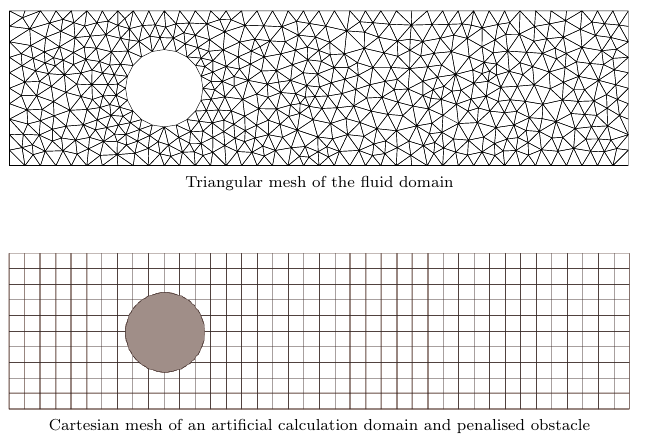
\includegraphics[width=.82\textwidth]{figures/ch07-fig02.png}
\caption{计算圆柱绕流的经典方法与罚方法.}
\label{fig:chap7-classic-penalty-meshes}
\end{figure}

在 $\mathcal U$ 中, 所考虑的方程是通常的 Navier--Stokes 方程; 而在障碍物内部, 由于系数 $\varepsilon$ 很小, 预期方程中的主导项为 $(1/\varepsilon^2)\chi_\omega u^\varepsilon$, 从而所考虑的方程将给出
\[
 \chi_\omega u^\varepsilon\approx\varepsilon^2.
\]
因此在渐近意义下, 可以认为当 $\varepsilon\to0$ 时 $u^\varepsilon$ 趋于 $0$. 最后, 我们希望在流体区域 $\mathcal U$ 中, $u^\varepsilon$ 接近物理解, 而后者当然没有定义在障碍物内.

从理论观点看, 文献\MBUnresolvedReference{bib:penalty-first-error-estimate}{[10]}首次建立了这一特定方法的误差估计. 这些估计与实验结果并不一致. 事实上, 该文献证明流体中的误差至少为 $\varepsilon^{1/2}$ 阶, 而数值结果似乎表明误差为 $\varepsilon$ 阶. 本节将按照文献\MBUnresolvedReference{bib:penalty-sharp-error}{[35, 37]}证明, 该方法产生的误差确实为 $\varepsilon$ 阶.

为实现这一目标, 同时这也是本节的第二个目标, 我们证明罚项的存在导致障碍物内部出现边界层, 但流体区域中不出现边界层. 对这个边界层的细致研究是证明精确误差估计的关键. 边界层理论在偏微分方程分析中非常重要, 对流体力学问题尤其如此. 这里的目标不是提出一般理论, 而只是通过一个来自数值问题的具体例子说明边界层概念.

我们拟按照 WKB 方法 (Wentzel--Kramers--Brillouin) 的思想, 对解进行渐近展开来证明边界层的存在性. 注意, 这种分析要求预先知道极限问题的解具有足够的正则性. 此外, 在当前情形中得到的是整体误差估计, 而不是只涉及流体区域的误差估计. 这就要求在低指标 Sobolev 空间中描述误差, 因为罚解不可能在整个计算区域 $\Omega$ 中都是光滑的.

为了说明所得结果在某种意义下是最优的, 同时也为了说明边界层概念和下文采用的技术, 本节一开始先描述一个简单的一维问题. 对这个玩具系统, 通过显式计算证明罚解与精确解之间的误差在 $L^2$ 范数下恰好为 $\varepsilon$ 阶.

\subsubsection{边界层的一个简单例子}
\label{subsec:chap7-simple-boundary-layer}

在开始研究上述问题之前, 先用一个例子说明, 当方程的一个参数趋于 $0$ 时, 描述边界层的方程会呈现怎样的行为.

考虑求解如下一维问题:
\begin{equation}
\left\{
\begin{aligned}
 -u''(x)&=1&&\text{于 } ]0,1[,\\
 u(0)&=u(1)=0.
\end{aligned}
\right.
\label{eq:chap7-one-dimensional-exact-problem}
\end{equation}
直接计算表明, 精确解为
\[
 u_0(x)=\frac12x(1-x).
\]

假设希望用与上述方法类似的罚方法求解该问题. 例如, 给定小参数 $\varepsilon$, 用如下罚问题代替问题\eqref{eq:chap7-one-dimensional-exact-problem}:
\begin{equation}
\left\{
\begin{aligned}
 -(u^\varepsilon)''(x)+\frac1{\varepsilon^2}\chi_{]-1,0[}u^\varepsilon&=1
 &&\text{于 } ]-1,1[,\\
 u^\varepsilon(-1)&=u^\varepsilon(1)=0.
\end{aligned}
\right.
\label{eq:chap7-one-dimensional-penalty-problem}
\end{equation}
若与导言中描述的模型作类比, 则计算区域为 $\Omega=]-1,1[$, 障碍物为 $\omega=]-1,0[$, 而``物理''区域为 $\mathcal U=\Omega\setminus\omega$.

现在计算近似问题的精确解, 并考察当 $\varepsilon$ 趋于零时它以何种方式收敛到初始问题的解 $u_0$. 为求解\eqref{eq:chap7-one-dimensional-penalty-problem}, 先分别在 $]-1,0[$ 和 $]0,1[$ 上求解. 此时在 $x=0$ 处尚无边界条件, 因而解的每一部分各有一个待定项. 直接计算后得到
\[
 u^\varepsilon(x)=
 \begin{cases}
  \dfrac12(1-x)(x+\beta),&x\in]0,1[,\\[4pt]
  A_0e^{-x/\varepsilon}+B_0e^{x/\varepsilon}-\varepsilon^2,&x\in]-1,0[,
 \end{cases}
\]
其中 $\beta,A_0,B_0$ 是待定常数. 边界条件 $u^\varepsilon(-1)=0$ 给出
\begin{equation}
 A_0e^{1/\varepsilon}+B_0e^{-1/\varepsilon}=\varepsilon^2.
\label{eq:chap7-one-dimensional-coefficient-one}
\end{equation}

现在必须写出连接解的两部分的条件. 已知\eqref{eq:chap7-one-dimensional-penalty-problem}的变分意义下解先验地定义于 $H_0^1(]-1,1[)$, 但若把方程写成
\[
 (u^\varepsilon)''=-1+\frac1{\varepsilon^2}\chi_{]-1,0[}u^\varepsilon
 \in L^2(]-1,1[),
\]
则可知该解实际上属于 $H^2(]-1,1[)$. 这意味着函数 $u^\varepsilon$ 及其导数 $(u^\varepsilon)'$ 在 $[-1,1]$ 上连续. 由此得到解的两部分之间的两个相容条件:
\begin{equation}
 \frac12\beta=A_0+B_0-\varepsilon^2,
\label{eq:chap7-one-dimensional-coefficient-two}
\end{equation}
\begin{equation}
 \frac12(1-\beta)=-\frac1\varepsilon A_0+\frac1\varepsilon B_0.
\label{eq:chap7-one-dimensional-coefficient-three}
\end{equation}
方程\eqref{eq:chap7-one-dimensional-coefficient-one}--\eqref{eq:chap7-one-dimensional-coefficient-three}给出常数 $\beta,A_0,B_0$ 关于 $\varepsilon$ 的表达式. 经过一些繁琐计算, 得
\[
\left\{
\begin{aligned}
 A_0&=\frac{\varepsilon^2(1+\varepsilon)-(\varepsilon^3+\varepsilon/2)e^{-1/\varepsilon}}
 {(1+\varepsilon)e^{1/\varepsilon}+(1-\varepsilon)e^{-1/\varepsilon}},\\
 B_0&=\frac{\varepsilon^2(1-\varepsilon)+(\varepsilon^3+\varepsilon/2)e^{1/\varepsilon}}
 {(1+\varepsilon)e^{1/\varepsilon}+(1-\varepsilon)e^{-1/\varepsilon}},\\
 \beta&=\frac{4\varepsilon^2-(2\varepsilon^2-\varepsilon)e^{1/\varepsilon}
 -(2\varepsilon^2+\varepsilon)e^{-1/\varepsilon}}
 {(1+\varepsilon)e^{1/\varepsilon}+(1-\varepsilon)e^{-1/\varepsilon}}.
\end{aligned}
\right.
\]
这些精确表达式本身意义不大. 回顾与 $\beta$ 不同, 常数 $A_0$ 和 $B_0$ 在 $u^\varepsilon$ 的表达式中位于指数项之前, 因而考察这些系数关于 $\varepsilon$ 的行为. 渐近地有
\[
 A_0\approx\varepsilon^2e^{-1/\varepsilon},\qquad
 B_0\approx\frac\varepsilon2,\qquad
 \beta\approx\varepsilon.
\]
因此在一阶近似下, 罚解 $u^\varepsilon$ 可表示为
\[
 u^\varepsilon(x)\approx
 \begin{cases}
  \varepsilon^2e^{-(1+x)/\varepsilon}+\dfrac\varepsilon2e^{x/\varepsilon}-\varepsilon^2,
  &x\in]-1,0[,\\[4pt]
  \dfrac12(1-x)(x+\varepsilon)=u_0(x)+\dfrac\varepsilon2(1-x),
  &x\in]0,1[.
 \end{cases}
\]
可见, 该方法在原区域 $]0,1[$ 中以 $\varepsilon$ 阶逼近初始问题的解 $u_0$, 且这对所有 Sobolev 范数均成立.

现在考察近似解在``障碍物''中的行为, 即在 $]-1,0[$ 中的行为 (见 Figures~\ref{fig:chap7-one-dimensional-penalty-solutions} 和~\ref{fig:chap7-one-dimensional-boundary-layer-zoom}). 它趋于零, 但仅在 $L^\infty$ 范数下如此. 事实上, 考察一阶导数的收敛性, 有
\[
 (u^\varepsilon)'(x)\approx-\varepsilon e^{-(1+x)/\varepsilon}
 +\frac12e^{x/\varepsilon},
\]
例如它在 $x=0$ 处趋于 $1/2$. 这是合理的, 因为精确解 $u_0$ 在 $x=0$ 处的导数值恰好是 $1/2$. 然而, 这会损害 $u^\varepsilon$ 在 $]-1,0[$ 中向 $0$ 在更高阶 Sobolev 空间中的收敛. 更准确地说, 有估计
\[
 \|u^\varepsilon\|_{L^2(]-1,0[)}\sim C\varepsilon^{3/2},\qquad
 \|(u^\varepsilon)'\|_{L^2(]-1,0[)}\sim C\sqrt\varepsilon,\qquad
 \|(u^\varepsilon)''\|_{L^2(]-1,0[)}\sim\frac C{\sqrt\varepsilon}.
\]
这种现象称为边界层, 因为近似解的导数在罚区域边界附近一个宽度为 $\varepsilon$ 的过渡区域中具有相对较大的值. 特别重要的是, 边界层只出现在被施加罚项的区域内部, 并不影响原区域 $]0,1[$ 内部的逼近.

下面将对不可压缩黏性流体绕障碍物流动的问题观察并描述同样的现象. 还将证明, 在这种情形下边界层也只出现在障碍物内部, 而不出现在流体区域. 此外, 在上述例子中可以看到边界层的尺度为 $\varepsilon$, 且解在该边界层内具有 $\varepsilon e^{-|x|/\varepsilon}$ 形式的行为.

正因如此, 在下文研究中寻找包含如下形式项的解的渐近展开:
\[
 W^0\left(t,x,\frac{d(x,\partial\omega)}\varepsilon\right),
\]
其中最后一个变量 (下文记作 $z$) 用来描述边界层内部的解.

\begin{figure}[H]
\centering
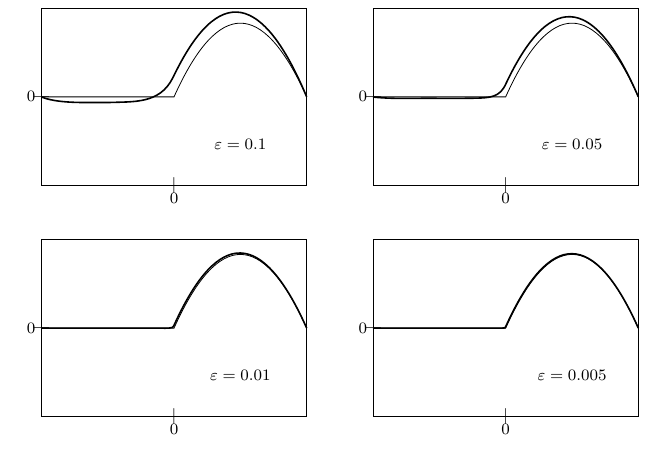
\includegraphics[width=.72\textwidth]{figures/ch07-fig03.png}
\caption{$\varepsilon=0.1,0.05,0.01,0.005$ 时精确解 (细线) 与罚解 (粗线) 的整体形状.}
\label{fig:chap7-one-dimensional-penalty-solutions}
\end{figure}

\begin{figure}[H]
\centering
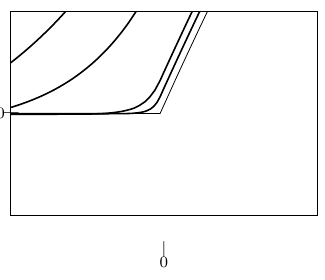
\includegraphics[width=.46\textwidth]{figures/ch07-fig04.png}
\caption{$x=0$ 处的放大图: $\varepsilon=0.1,0.05,0.01,0.005$ 时的精确解 (细线) 与罚解 (粗线).}
\label{fig:chap7-one-dimensional-boundary-layer-zoom}
\end{figure}

\par\noindent\refstepcounter{chaptersevensectiontworemark}\textbf{Remark~\thechaptersevensectiontworemark:}\label{rem:chap7-artificial-boundary-condition}
在这个问题中, $x=-1$ 处所选的人工边界条件几乎并不重要. 因此, 若把 Dirichlet 边界条件替换为 Neumann 型边界条件
\[
 (u^\varepsilon)'(-1)=0,
\]
则解的一般公式保持不变, 但 $A_0,B_0,\beta$ 所满足的关系现在是\eqref{eq:chap7-one-dimensional-coefficient-two}、\eqref{eq:chap7-one-dimensional-coefficient-three}, 以及 $x=-1$ 处替代\eqref{eq:chap7-one-dimensional-coefficient-one}的新条件
\[
 -\frac{A_0}\varepsilon e^{1/\varepsilon}
 +\frac{B_0}\varepsilon e^{-1/\varepsilon}=0.
\]
于是可以证明有如下渐近关系:
\[
 A_0\approx\varepsilon e^{-2/\varepsilon},\qquad
 B_0\approx\frac\varepsilon2,\qquad
 \beta\approx\varepsilon.
\]
因而在 $[-1,0]$ 上,
\[
 u^\varepsilon(x)\approx\varepsilon^2e^{-(x+2)/\varepsilon}
 +\frac\varepsilon2e^{x/\varepsilon}-\varepsilon^2.
\]
解的整体行为因此与上面观察到的行为相同.

\subsubsection{主要结果的陈述}
\label{subsec:chap7-penalty-main-result}

现在可以陈述关于障碍物周围 Navier--Stokes 方程罚方法的主要结果. 为简化计算, 假设 Reynolds 数等于 $1$. 这是合理的, 因为此处关注的不是黏性边界层 (在无黏极限 $\operatorname{Re}\to0$ 中可以观察到它), 而是罚方法所诱导的边界层. 此外, 将证明这一边界层只在被施加罚项的障碍物内部发展, 因而不会干扰流体区域中形成的特征尺度为 $\sqrt{\operatorname{Re}}$ 的黏性边界层.

本节始终用 $\Omega$ 表示 $\mathbb R^d$ 中光滑有界区域 (至少为 $C^{5,1}$ 类), $d=2$ 或 $3$; $\omega$ 是 $\Omega$ 的有界子区域, 与 $\Omega$ 具有相同正则性, 且 $\overline\omega\subset\Omega$. 记流体区域为 $\mathcal U=\Omega\setminus\overline\omega$. 在此框架下, 首先回顾 Navier--Stokes 方程解的存在性与正则性结果 (Theorems~\ref{thm:chap5-strong-solutions}, \ref{thm:chap5-parabolic-regularity} 和 Corollary~\ref{cor:chap5-parabolic-time-continuity}).

\begin{figure}[H]
\centering
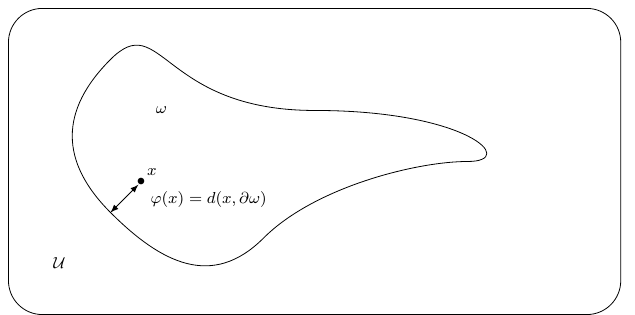
\includegraphics[width=.72\textwidth]{figures/ch07-fig05.png}
\caption{包含流体区域 $\mathcal U$ 和障碍物 $\omega$ 的计算区域 $\Omega$.}
\label{fig:chap7-fluid-obstacle-domain}
\end{figure}

\begin{Proposition}
\label{prop:chap7-limit-fluid-strong-solution}
设 $v_0\in(H^5(\mathcal U))^d\cap V$, 且
$f\in C^2([0,+\infty[,(H^4(\mathcal U))^d)$ 满足相容性条件\eqref{eq:chap5-parabolic-compatibility}. 则存在终止时间 $T^*>0$, 以及定义于 $[0,T^*[\times\mathcal U$ 上的唯一二元组 $(V^0,p^0)$, 满足
\[
\left\{
\begin{aligned}
 \frac{\partial V^0}{\partial t}-\Delta V^0+(V^0\cdot\nabla)V^0+\nabla p^0&=f
 &&\text{于 }\mathcal U,\\
 \operatorname{div}V^0&=0&&\text{于 }\mathcal U,\\
 V^0&=0&&\text{于 }\partial\mathcal U,\\
 V^0(0)&=v_0,
\end{aligned}
\right.
\]
并且对所有 $T<T^*$,
\begin{equation}
\left\{
\begin{aligned}
 V^0&\in C^0([0,T],(H^5(\mathcal U))^d)
 \cap L^2(]0,T[,(H^6(\mathcal U))^d),\\
 \frac{\partial V^0}{\partial t}&\in C^0([0,T],(H^3(\mathcal U))^d)
 \cap L^2(]0,T[,(H^4(\mathcal U))^d),\\
 \frac{\partial^2V^0}{\partial t^2}&\in C^0([0,T],(H^1(\mathcal U))^d)
 \cap L^2(]0,T[,(H^2(\Omega))^d),\\
 p^0&\in C^0([0,T],H^4(\mathcal U))
 \cap L^2(]0,T[,H^5(\mathcal U)),\\
 \frac{\partial p^0}{\partial t}&\in C^0([0,T],H^2(\mathcal U))
 \cap L^2(]0,T[,H^3(\mathcal U)).
\end{aligned}
\right.
\label{eq:chap7-limit-fluid-regularity}
\end{equation}
此外, 在维数 $d=2$ 的情形下, $T^*=+\infty$.
\end{Proposition}

因此, 我们提出用区域 $\Omega$ 中问题\eqref{eq:chap7-penalized-navier-stokes}的解 $u^\varepsilon$ 的数值计算, 替代流体区域 $\mathcal U$ 中 $V^0$ 的数值计算. 随后将证明一个误差估计, 它给出这一方法所造成误差的精确量级. 更准确地说, 有如下结果.

\begin{Theorem}
\label{thm:chap7-penalty-error}
设 $v_0,f,V^0,T^*$ 如 Proposition~\ref{prop:chap7-limit-fluid-strong-solution} 中所述. 定义如下形式的初始数据扰动:
\[
 u_0^\varepsilon(x)=
 \begin{cases}
  v_0(x)+r_0^\varepsilon(x),&x\in\mathcal U,\\
  r_0^\varepsilon(x),&x\in\omega,
 \end{cases}
\]
其中 $\operatorname{div}r_0^\varepsilon=0$, 且
$\|r_0^\varepsilon\|_{L^2(\Omega)}\leq K\varepsilon$. 则存在罚问题
\[
\left\{
\begin{aligned}
 \frac{\partial u^\varepsilon}{\partial t}-\Delta u^\varepsilon
 +(u^\varepsilon\cdot\nabla)u^\varepsilon+\nabla\pi^\varepsilon
 +\frac1{\varepsilon^2}\chi_\omega u^\varepsilon&=f&&\text{于 }\Omega,\\
 \operatorname{div}u^\varepsilon&=0&&\text{于 }\Omega,\\
 u^\varepsilon&=0&&\text{于 }\partial\Omega,\\
 u^\varepsilon(0)&=u_0^\varepsilon
\end{aligned}
\right.
\]
的弱解 $(u^\varepsilon,\pi^\varepsilon)$, 使得对所有 $T<T^*$, 存在与 $\varepsilon$ 无关的常数 $C$, 满足
\[
 \|u^\varepsilon\|_{L^\infty(]0,T[,(L^2(\Omega))^d)}
 +\|u^\varepsilon\|_{L^2(]0,T[,(H_0^1(\Omega))^d)}\leq C.
\]
此外, 在 $\mathcal U$ 中, $u^\varepsilon$ 在能量范数下是 $V^0$ 的一阶逼近. 这意味着对所有 $T<T^*$, 存在 $C>0$, 使
\[
 \|u^\varepsilon-V^0\|_{L^\infty(]0,T[,(L^2(\mathcal U))^d)}
 +\|u^\varepsilon-V^0\|_{L^2(]0,T[,(H^1(\mathcal U))^d)}
 \leq C\varepsilon.
\]
最后, $(u^\varepsilon)_\varepsilon$ 在 $\omega$ 中按如下意义趋于零:
\[
 \|u^\varepsilon\|_{L^\infty(]0,T[,(L^2(\omega))^d)}\leq C\varepsilon,
 \qquad
 \|u^\varepsilon\|_{L^2(]0,T[,(H^1(\omega))^d)}\leq C\sqrt\varepsilon.
\]
\end{Theorem}

对给定的 $\varepsilon>0$, 解 $u^\varepsilon$ 的存在性所涉及的技术与 Chapter~\ref{chap:homogeneous-navier-stokes} 中介绍的技术相同. 在维数 $2$ 下, 该解唯一. 难点在于建立误差估计. 为证明这一结果, 对解 $u^\varepsilon$ 进行渐近展开, 从而描述障碍物 $\omega$ 内部存在的边界层.

假设 $\omega$ 足够正则, 因而已知 (见 Chapter~\ref{chap:sobolev-spaces} Section~\ref{subsec:chap3-boundary-distance-projection}) 在 $\omega$ 中存在 $\partial\omega$ 的一个邻域
\[
 \omega_1=\{x\in\omega,\ d(x,\partial\omega)<\eta\},
\]
函数 $x\mapsto\delta(x)=d(x,\partial\omega)$ 在其中光滑. 因而在下文中固定一个 $\omega$ 上的正则函数 $\varphi$, 它在 $\omega_1$ 上与 $\delta$ 重合. 注意在 $\partial\omega$ 上,
$\nabla\varphi=\nabla\delta=\nu$, 其中 $\nu$ 是 $\omega$ 的向内单位法向, 同时由于 $\omega$ 和 $\mathcal U$ 共有一部分边界, 它也是 $\mathcal U$ 在 $\partial\omega$ 上的向外单位法向.

此外, 对任意 $x\in\omega_1$, 有
$\nabla\varphi(x)=\nu(P_0(x))$, 其中 $P_0(x)$ 是 $x$ 在 $\partial\omega$ 上的正交投影, 见\eqref{eq:chap3-distance-gradient-normal}. 特别地, 在 $\omega_1$ 中 $|\nabla\varphi|=1$.

现在可如下描述边界层.

\begin{Theorem}
\label{thm:chap7-penalty-boundary-layer-expansion}
设 $v_0,f,V^0,T^*$ 如 Proposition~\ref{prop:chap7-limit-fluid-strong-solution} 中所述. 存在定义于 $[0,T^*[\times\mathcal U$ 上的两个函数 $V^1,V^2$, 以及定义于 $[0,T^*[\times\omega\times\mathbb R^+$ 上的两个函数 $W^1,W^2$, 它们足够光滑, 使得
\[
 u^\varepsilon(t,x)=
 \begin{cases}
  V^0(t,x)+\varepsilon V^1(t,x)+\varepsilon^2V^2(t,x)
  +\varepsilon v_\varepsilon^r(t,x),&x\in\mathcal U,\\[3pt]
  \varepsilon W^1\left(t,x,\dfrac{\varphi(x)}\varepsilon\right)
  +\varepsilon^2W^2\left(t,x,\dfrac{\varphi(x)}\varepsilon\right)
  +\varepsilon w_\varepsilon^r(t,x),&x\in\omega,
 \end{cases}
\]
其中对所有 $T<T^*$, $v_\varepsilon^r$ 和 $w_\varepsilon^r$ 在
$L^\infty(]0,T[,(L^2)^d)\cap L^2(]0,T[,(H^1)^d)$ 中具有与 $\varepsilon$ 无关的界.
\end{Theorem}

Theorem~\ref{thm:chap7-penalty-error} 给出的误差估计现在是 Theorem~\ref{thm:chap7-penalty-boundary-layer-expansion} 的直接推论. 后者实际上更精确, 因为它完整描述了 $\omega$ 中边界层的第一项.

寻找上述多尺度形式的渐近展开 (即引入变量 $\varphi/\varepsilon$) 称为 WKB 方法. 首先找出各轮廓必须满足的方程. 然后证明所得渐近展开各项的存在性和正则性. 最后在末节估计余项大小并证明收敛性.

\par\noindent\refstepcounter{chaptersevensectiontworemark}\textbf{Remark~\thechaptersevensectiontworemark:}\label{rem:chap7-second-order-wkb-necessity}
由下面对函数 $V^1,V^2,W^1,W^2$ 的定义, 可能会预期余项 $\varepsilon v_\varepsilon^r$ 和 $\varepsilon w_\varepsilon^r$ 至少具有 $\varepsilon^2$ 的量级. 正如通常观察到的那样, WKB 轮廓分解方法并不必然给出这一结果. 例如与文献\MBUnresolvedReference{bib:wkb-remainder-one}{[32]}或\MBUnresolvedReference{bib:wkb-remainder-two}{[38]}中相同, 为证明余项为 $\varepsilon$ 阶, 绝对有必要把形式展开写到二阶项.

\subsubsection{形式渐近展开}
\label{subsec:chap7-formal-asymptotic-expansion}

为构造渐近展开, 采用充分条件进行处理. 该展开尤其依赖于 $\varphi$ 的选择, 而我们并不关心它在边界层之外的唯一性. 该展开的唯一目标是在足够高阶上构造问题的一个显式近似解.

因此, 设 $u^\varepsilon$ 是如下问题之解:
\begin{equation}
\left\{
\begin{aligned}
 \frac{\partial u^\varepsilon}{\partial t}-\Delta u^\varepsilon
 +(u^\varepsilon\cdot\nabla)u^\varepsilon+\nabla\pi^\varepsilon
 +\frac1{\varepsilon^2}\chi_\omega u^\varepsilon&=f&&\text{于 }\Omega,\\
 \operatorname{div}u^\varepsilon&=0&&\text{于 }\Omega,\\
 u^\varepsilon&=0&&\text{于 }\partial\Omega,\\
 u^\varepsilon(0,x)&=u_0^\varepsilon(x).
\end{aligned}
\right.
\label{eq:chap7-penalty-asymptotic-problem}
\end{equation}

首先要区分解在障碍物 $\omega$ 内部的行为与它在流体区域 $\mathcal U$ 中的行为. 为此, 分别用 $v^\varepsilon$ 和 $p^\varepsilon$ 表示 $u^\varepsilon$ 和 $\pi^\varepsilon$ 在 $\mathcal U=\Omega\setminus\overline\omega$ 上的限制, 并分别用 $w^\varepsilon$ 和 $q^\varepsilon$ 表示 $u^\varepsilon$ 和 $\pi^\varepsilon$ 在 $\omega$ 上的限制. 于是整体问题\eqref{eq:chap7-penalty-asymptotic-problem}等价于函数 $v^\varepsilon,w^\varepsilon,p^\varepsilon,q^\varepsilon$ 所满足的如下系统
\begin{equation}
\left\{
\begin{alignedat}{3}
 \frac{\partial w^\varepsilon}{\partial t}-\Delta w^\varepsilon
 +(w^\varepsilon\cdot\nabla)w^\varepsilon+\nabla q^\varepsilon
 +\frac1{\varepsilon^2}w^\varepsilon&=0&&\quad\text{于 }\omega,&&(1)\\
 \operatorname{div}w^\varepsilon&=0&&\quad\text{于 }\omega,&&(2)\\
 \frac{\partial v^\varepsilon}{\partial t}-\Delta v^\varepsilon
 +(v^\varepsilon\cdot\nabla)v^\varepsilon+\nabla p^\varepsilon&=f&&\quad\text{于 }\mathcal U,&&(3)\\
 \operatorname{div}v^\varepsilon&=0&&\quad\text{于 }\mathcal U,&&(4)\\
 v^\varepsilon&=w^\varepsilon&&\quad\text{于 }\partial\omega,&&(5)\\
 -\frac{\partial v^\varepsilon}{\partial\nu}+p^\varepsilon\nu
 &=-\frac{\partial w^\varepsilon}{\partial\nu}+q^\varepsilon\nu
 &&\quad\text{于 }\partial\omega,&&(6)\\
 v^\varepsilon&=0&&\quad\text{于 }\partial\Omega.&&(7)
\end{alignedat}
\right.
\label{eq:chap7-penalty-transmission-system}
\end{equation}

\par\noindent\refstepcounter{chaptersevensectiontworemark}\textbf{Remark~\thechaptersevensectiontworemark:}\label{rem:chap7-natural-transmission-conditions}
前一系统中的边界条件 (5) 和 (6) 是自然传递条件, 它们保证 $u^\varepsilon$ 的迹以及法向通量 $(\pi^\varepsilon-\nabla u^\varepsilon)\mathbin{.}\nu$ 穿过 $\partial\omega$ 时在迹的意义下连续, 从而保证存在属于 $(H^2(\Omega))^d$ 的解 $u^\varepsilon$. 例如, 为论证通量传递条件, 可按如下方式进行.

取无散试验函数 $\psi\in(\mathcal D(\Omega))^d$, 并利用 $f$ 在 $\omega$ 上由 $0$ 延拓这一事实, 写出\eqref{eq:chap7-penalty-asymptotic-problem}的弱形式,
\[
 \frac d{dt}\int_\Omega u^\varepsilon\cdot\psi\,dx
 +\int_\Omega\nabla u^\varepsilon:\nabla\psi\,dx
 +\int_\Omega((u^\varepsilon\cdot\nabla)u^\varepsilon)\cdot\psi\,dx
 +\frac1{\varepsilon^2}\int_\omega u^\varepsilon\cdot\psi\,dx
 =\int_\mathcal U f\cdot\psi\,dx.
\]
然后将障碍物内部的方程 (1) 乘以 $\psi|_\omega$, 后者在 $\partial\omega$ 上当然不为零, 并且由于 $\nu$ 是 $\omega$ 的向内法向, 分部积分给出
\[
\begin{aligned}
 &\frac d{dt}\int_\omega w^\varepsilon\cdot\psi\,dx
 +\int_\omega\nabla w^\varepsilon:\nabla\psi\,dx
 +\int_{\partial\omega}\left(+\frac{\partial w^\varepsilon}{\partial\nu}-q^\varepsilon\nu\right)\cdot\psi\,d\sigma\\
 &\qquad+\int_\omega((w^\varepsilon\cdot\nabla)w^\varepsilon)\cdot\psi\,dx
 +\frac1{\varepsilon^2}\int_\omega w^\varepsilon\cdot\psi\,dx=0,
\end{aligned}
\]
再将流体中的方程 (3) 乘以 $\psi|_\mathcal U$. 这给出
\[
 \frac d{dt}\int_\mathcal U v^\varepsilon\cdot\psi\,dx
 +\int_\mathcal U\nabla v^\varepsilon:\nabla\psi\,dx
 +\int_{\partial\omega}\left(-\frac{\partial v^\varepsilon}{\partial\nu}+p^\varepsilon\nu\right)\cdot\psi\,d\sigma
 +\int_\mathcal U((v^\varepsilon\cdot\nabla)v^\varepsilon)\cdot\psi\,dx
 =\int_\mathcal U f\cdot\psi\,dx.
\]
现在将最后两个等式相加, 并将所得结果与第一个等式比较, 同时回忆 $v^\varepsilon$ 和 $w^\varepsilon$ 分别是 $u^\varepsilon$ 在 $\mathcal U$ 和 $\omega$ 上的限制. 于是剩下
\[
 \int_{\partial\omega}\left(+\frac{\partial w^\varepsilon}{\partial\nu}-q^\varepsilon\nu\right)\cdot\psi\,d\sigma
 +\int_{\partial\omega}\left(-\frac{\partial v^\varepsilon}{\partial\nu}+p^\varepsilon\nu\right)\cdot\psi\,d\sigma=0.
\]
此关系必须对所有试验函数 $\psi$ 成立, 这就证明了方程 (6).

寻找 $v^\varepsilon,w^\varepsilon,p^\varepsilon,q^\varepsilon$ 的如下形式的渐近展开 (这称为一个 ansatz)
\begin{equation}
\left\{
\begin{aligned}
 v^\varepsilon(t,x)&=V^0(t,x)+\varepsilon V^1(t,x)+\cdots,\\
 p^\varepsilon(t,x)&=\frac1{\varepsilon^2}p^{-2}(t,x)+\frac1\varepsilon p^{-1}(t,x)+p^0(t,x)+\cdots,\\
 w^\varepsilon(t,x)&=W^0\left(t,x,\frac{\varphi(x)}\varepsilon\right)
 +\varepsilon W^1\left(t,x,\frac{\varphi(x)}\varepsilon\right)+\cdots,\\
 q^\varepsilon(t,x)&=\frac1{\varepsilon^2}q^{-2}\left(t,x,\frac{\varphi(x)}\varepsilon\right)
 +\frac1\varepsilon q^{-1}\left(t,x,\frac{\varphi(x)}\varepsilon\right)
 +q^0\left(t,x,\frac{\varphi(x)}\varepsilon\right)+\cdots.
\end{aligned}
\right.
\label{eq:chap7-penalty-profile-ansatz}
\end{equation}
此外, 正如在本节开头所考察的一维例子中看到的那样, 在障碍物内部将各轮廓项寻找为如下形式是合理的:
\[
 W^i(t,x,z)=\overline W^i(t,x)+\widetilde W^i(t,x,z),
 \qquad q^i(t,x,z)=\overline q^i(t,x)+\widetilde q^i(t,x,z),
\]
其中 $\overline W^i$ 和 $\overline q^i$ 是轮廓的内部项, 即不对边界层作出贡献的项, 相反 $\widetilde W^i$ 和 $\widetilde q^i$ 描述边界层内部的行为. 这确切地意味着, 对 $\omega$ 中固定的 $x$, 应有 $\lim_{\varepsilon\to0}\widetilde W^i(t,x,\varphi(x)/\varepsilon)=0$. 再次受到 Section~\ref{subsec:chap7-simple-boundary-layer} 中一维例子的启发, 在那里得到形如 $g(x)e^{-|x|/\varepsilon}$ 的边界层轮廓, 我们预期轮廓 $\widetilde W^i$ 和 $\widetilde q^i$ 关于标量变量 $z$ 的衰减非常迅速.

因此, 下文将施加条件: $\widetilde W^i$ 和 $\widetilde q^i$ 以及它们关于 $z$ 的导数在 $z$ 趋于无穷时趋于 $0$; 即对任意 $i$ 和 $k\geq0$,
\begin{equation}
 \partial_z^k\widetilde W^i\underset{z\to+\infty}{\longrightarrow}0
 \quad\text{且}\quad
 \partial_z^k\widetilde q^i\underset{z\to+\infty}{\longrightarrow}0,
 \qquad\forall(t,x)\in[0,T^*[\times\omega.
\label{eq:chap7-profile-decay-condition}
\end{equation}

最后将证明, 确实能够构造满足这一假设的轮廓, 并且如所预期的那样, 关于 $z$ 的衰减是指数型的.

\paragraph{轮廓方程的确定}
\label{subsubsec:chap7-determining-profile-equations}

下文对函数 $W(t,x,z)$ 使用的微分算子标准记号 $\nabla$, $\operatorname{div}$, $\Delta$ 表示仅作用于原空间变量 $x$ 的算子. 用 $W_z,W_{zz}$ 等表示关于边界层变量 $z$ 的导数.

因此, 对任意向量场 $(t,x,z)\mapsto W(t,x,z)$, 由 $(t,x)\mapsto w(t,x)=W(t,x,\varphi(x)/\varepsilon)$ 定义的函数满足公式
\begin{equation}
\left\{
\begin{aligned}
 \nabla w&=\nabla W+\frac1\varepsilon W_z\otimes\nabla\varphi,\\
 \operatorname{div}w&=\operatorname{div}W+\frac1\varepsilon W_z\cdot\nabla\varphi,\\
 \Delta w&=\Delta W+\frac2\varepsilon\nabla W_z\mathbin{.}\nabla\varphi
 +\frac1\varepsilon(\Delta\varphi)W_z
 +\frac1{\varepsilon^2}|\nabla\varphi|^2W_{zz},
\end{aligned}
\right.
\label{eq:chap7-boundary-layer-differential-formulas}
\end{equation}
而对任意标量函数 $(t,x,z)\mapsto\Pi(t,x,z)$, 函数 $(t,x)\mapsto\pi(t,x)=\Pi(t,x,\varphi(x)/\varepsilon)$ 满足
\[
 \nabla\pi=\nabla\Pi+\frac1\varepsilon\Pi_z\nabla\varphi.
\]
最后回忆, 在 $\omega_1$ 中函数 $\varphi$ 满足 $|\nabla\varphi|=1$, 并且在边界 $\partial\omega$ 上有 $\nabla\varphi=\nu$, 即流体区域 $\mathcal U$ 的向外法向, 它也是障碍物 $\omega$ 的向内法向.

现在的一般原则如下: 将形式表达式\eqref{eq:chap7-penalty-profile-ansatz}代入方程\eqref{eq:chap7-penalty-transmission-system}, 后者已经写成关于 $x$ 和 $z$ 的导数的函数; 然后形式地逐个比较 $\varepsilon$ 的各次幂所对应的项, 边界条件中也如此.

\subparagraph{方程\eqref{eq:chap7-penalty-transmission-system}中方程 (1) 的渐近展开}

\begin{itemize}
\item $\varepsilon^{-2}$ 阶:
\[
 -W^0_{zz}+W^0+q^{-1}_z\nabla\varphi=0,
\]
因此, 利用假设\eqref{eq:chap7-profile-decay-condition}, 令此方程中的 $z$ 趋于 $+\infty$, 得
\begin{equation}
 \overline W^0=0,\qquad\text{于 }\omega,
\label{eq:chap7-interior-W0-zero}
\end{equation}
并且作差得到
\begin{equation}
 -\widetilde W^0_{zz}+\widetilde W^0+\widetilde q^{-1}_z\nabla\varphi=0,
 \qquad\text{于 }\omega\times\mathbb R^+.
\label{eq:chap7-boundary-W0-equation}
\end{equation}

\item $\varepsilon^{-1}$ 阶:
\[
 -W^1_{zz}+W^1-2\nabla W^0_z\mathbin{.}\nabla\varphi
 -(\Delta\varphi)W^0_z+(W^0\cdot\nabla\varphi)W^0_z
 +\nabla q^{-1}+q^0_z\nabla\varphi=0;
\]
因此再次利用假设\eqref{eq:chap7-profile-decay-condition}, 当 $z$ 趋于无穷时得到
\begin{equation}
 \overline W^1+\nabla\overline q^{-1}=0,\qquad\text{于 }\omega,
\label{eq:chap7-interior-W1-equation}
\end{equation}
而与上式作差给出
\begin{equation}
\begin{split}
 -\widetilde W^1_{zz}+\widetilde W^1
 -2(\nabla\varphi\cdot\nabla\widetilde W^0_z)
 -(\Delta\varphi)\widetilde W^0_z
 +(W^0\cdot\nabla\varphi)\widetilde W^0_z\\
 {}+\nabla\widetilde q^{-1}+\widetilde q^0_z\nabla\varphi=0,
 \qquad\text{于 }\omega\times\mathbb R^+.
\end{split}
\label{eq:chap7-boundary-W1-equation}
\end{equation}

\item $\varepsilon^0$ 阶:
\[
\begin{split}
 \frac{\partial W^0}{\partial t}-W^2_{zz}-2\nabla W^1_z\mathbin{.}\nabla\varphi
 -(\Delta\varphi)W^1_z-\Delta W^0+(W^0\cdot\nabla)W^0\\
 {}+(W^1\cdot\nabla\varphi)W^0_z+(W^0\cdot\nabla\varphi)W^1_z
 +\nabla q^0+q^1_z\nabla\varphi+W^2=0,
 \qquad\text{于 }\omega\times\mathbb R^+.
\end{split}
\]
因此再次令 $z$ 趋于 $+\infty$, 得
\begin{equation}
 \frac{\partial\overline W^0}{\partial t}-\Delta\overline W^0
 +(\overline W^0\cdot\nabla)\overline W^0+\nabla\overline q^0+\overline W^2=0,
 \qquad\text{于 }\omega,
\label{eq:chap7-interior-W2-equation}
\end{equation}
并且再次作差得到
\begin{equation}
\begin{split}
 \frac{\partial\widetilde W^0}{\partial t}-\widetilde W^2_{zz}
 -2\nabla\widetilde W^1_z\mathbin{.}\nabla\varphi
 -(\Delta\varphi)\widetilde W^1_z-\Delta\widetilde W^0
 +(\widetilde W^0\cdot\nabla)\overline W^0
 +(W^0\cdot\nabla)\widetilde W^0\\
 {}+(W^1\cdot\nabla\varphi)\widetilde W^0_z
 +(W^0\cdot\nabla\varphi)\widetilde W^1_z
 +\nabla\widetilde q^0+\widetilde q^1_z\nabla\varphi+\widetilde W^2=0,
 \qquad\text{于 }\omega\times\mathbb R^+.
\end{split}
\label{eq:chap7-boundary-W2-equation}
\end{equation}

\item $\varepsilon$ 阶:
在 $\omega\times\mathbb R^+$ 中这给出
\[
\begin{split}
 \frac{\partial W^1}{\partial t}-W^3_{zz}-2\nabla W^2_z\mathbin{.}\nabla\varphi
 -(\Delta\varphi)W^2_z-\Delta W^1+(W^0\cdot\nabla)W^1+(W^1\cdot\nabla)W^0\\
 {}+(W^0\cdot\nabla\varphi)W^2_z+(W^1\cdot\nabla\varphi)W^1_z
 +(W^2\cdot\nabla\varphi)W^0_z+\nabla q^1+q^2_z\nabla\varphi+W^3=0.
\end{split}
\]
当 $z$ 趋于无穷时, 在 $\omega\times\mathbb R^+$ 中得到
\begin{equation}
 \frac{\partial\overline W^1}{\partial t}-\Delta\overline W^1
 +(\overline W^0\cdot\nabla)\overline W^1
 +(\overline W^1\cdot\nabla)\overline W^0
 +\nabla\overline q^1+\overline W^3=0.
\label{eq:chap7-interior-W3-equation}
\end{equation}
\end{itemize}

\subparagraph{方程\eqref{eq:chap7-penalty-transmission-system}中方程 (2) 的渐近展开}

\begin{itemize}
\item $\varepsilon^{-1}$ 阶:
\begin{equation}
 \widetilde W^0_z\cdot\nabla\varphi=0,
 \qquad\text{于 }\omega\times\mathbb R^+.
\label{eq:chap7-boundary-W0-normal-zero}
\end{equation}

\item $\varepsilon^0$ 阶:
\[
 \nabla\varphi\cdot W^1_z+\operatorname{div}W^0=0,
\]
因而
\begin{equation}
 \operatorname{div}\overline W^0=0,\qquad\text{于 }\omega,
\label{eq:chap7-interior-W0-divergence}
\end{equation}
\begin{equation}
 \nabla\varphi\cdot\widetilde W^1_z+\operatorname{div}\widetilde W^0=0,
 \qquad\text{于 }\omega\times\mathbb R^+.
\label{eq:chap7-boundary-W1-divergence}
\end{equation}

\item $\varepsilon$ 阶:
\[
 \nabla\varphi\cdot W^2_z+\operatorname{div}W^1=0;
\]
因而
\begin{equation}
 \operatorname{div}\overline W^1=0,\qquad\text{于 }\omega,
\label{eq:chap7-interior-W1-divergence}
\end{equation}
\begin{equation}
 \nabla\varphi\cdot\widetilde W^2_z+\operatorname{div}\widetilde W^1=0,
 \qquad\text{于 }\omega\times\mathbb R^+.
\label{eq:chap7-boundary-W2-divergence}
\end{equation}

\item $\varepsilon^2$ 阶:
\[
 \nabla\varphi\cdot W^3_z+\operatorname{div}W^2=0;
\]
因此当 $z$ 趋于无穷时有
\begin{equation}
 \operatorname{div}\overline W^2=0,\qquad\text{于 }\omega.
\label{eq:chap7-interior-W2-divergence}
\end{equation}

\item $\varepsilon^3$ 阶:
\[
 \nabla\varphi\cdot W^4_z+\operatorname{div}W^3=0;
\]
因此与前面相同,
\begin{equation}
 \operatorname{div}\overline W^3=0,\qquad\text{于 }\omega.
\label{eq:chap7-interior-W3-divergence}
\end{equation}
\end{itemize}

\subparagraph{方程\eqref{eq:chap7-penalty-transmission-system}中方程 (3) 的渐近展开}

\begin{itemize}
\item $\varepsilon^0$ 阶:
\begin{equation}
 \frac{\partial V^0}{\partial t}-\Delta V^0+(V^0\cdot\nabla)V^0+\nabla p^0=f,
 \qquad\text{于 }\mathcal U.
\label{eq:chap7-fluid-V0-equation}
\end{equation}

\item $\varepsilon^1$ 阶:
\begin{equation}
 \frac{\partial V^1}{\partial t}-\Delta V^1+(V^0\cdot\nabla)V^1
 +(V^1\cdot\nabla)V^0+\nabla p^1=0,
 \qquad\text{于 }\mathcal U.
\label{eq:chap7-fluid-V1-equation}
\end{equation}

\item $\varepsilon^2$ 阶:
\begin{equation}
 \frac{\partial V^2}{\partial t}-\Delta V^2+(V^0\cdot\nabla)V^2
 +(V^1\cdot\nabla)V^1+(V^2\cdot\nabla)V^0+\nabla p^2=0,
 \qquad\text{于 }\mathcal U.
\label{eq:chap7-fluid-V2-equation}
\end{equation}
\end{itemize}

\subparagraph{方程\eqref{eq:chap7-penalty-transmission-system}中方程 (4) 的渐近展开}

在所有阶上得到关系
\begin{equation}
 \operatorname{div}V^0=\operatorname{div}V^1=\operatorname{div}V^2=0,
 \qquad\text{于 }\mathcal U.
\label{eq:chap7-fluid-profile-divergence}
\end{equation}

\subparagraph{方程\eqref{eq:chap7-penalty-transmission-system}中方程 (5) 的渐近展开}

容易得到关系
\begin{equation}
 V^0=W^0,\qquad V^1=W^1,\qquad V^2=W^2,
 \qquad\text{于 }\partial\omega\times\{z=0\}.
\label{eq:chap7-profile-value-transmission}
\end{equation}

\subparagraph{方程\eqref{eq:chap7-penalty-transmission-system}中方程 (6) 的渐近展开}

\begin{itemize}
\item $\varepsilon^{-1}$ 阶:
\begin{equation}
 -W^0_z+q^{-1}\nu=0,
 \qquad\text{于 }\partial\omega\times\{z=0\}.
\label{eq:chap7-profile-flux-order-minus-one}
\end{equation}

\item $\varepsilon^0$ 阶:
\begin{equation}
 -\frac{\partial W^0}{\partial\nu}-W^1_z+q^0\nu
 =p^0\nu-\frac{\partial V^0}{\partial\nu},
 \qquad\text{于 }\partial\omega\times\{z=0\}.
\label{eq:chap7-profile-flux-order-zero}
\end{equation}

\item $\varepsilon$ 阶:
\begin{equation}
 -\frac{\partial W^1}{\partial\nu}-W^2_z+q^1\nu
 =p^1\nu-\frac{\partial V^1}{\partial\nu},
 \qquad\text{于 }\partial\omega\times\{z=0\}.
\label{eq:chap7-profile-flux-order-one}
\end{equation}
\end{itemize}

\paragraph{轮廓方程的形式求解}
\label{subsubsec:chap7-formal-profile-resolution}

现在暂时在形式层面确定渐近展开的各项. 使用上面通过比较原方程中 $\varepsilon$ 的各次幂所得的关系, 并寻找这些方程的解. 注意其中一些方程没有唯一解, 因而任意选择一个可能的解. 如果回忆起主要目标是得到一个适当的近似解, 而这样的近似解当然并不唯一, 这一点并不令人意外.

\subparagraph{$q^{-1}$ 和 $\overline W^1$ 的确定}

将\eqref{eq:chap7-profile-flux-order-minus-one}与 $\nabla\varphi$ 作标量积, 由于 $\widetilde W^0_z\cdot\nabla\varphi=0$ (见\eqref{eq:chap7-boundary-W0-normal-zero}), 并且在 $\partial\omega$ 上 $\nabla\varphi=\nu$, 得
\begin{equation}
 q^{-1}=0,\qquad\text{于 }\partial\omega\times\{z=0\}.
\label{eq:chap7-qminusone-boundary-zero}
\end{equation}
现在对\eqref{eq:chap7-interior-W1-equation}取散度并使用\eqref{eq:chap7-interior-W1-divergence}, 得
\begin{equation}
 \Delta\overline q^{-1}=0,\qquad\text{于 }\omega.
\label{eq:chap7-qminusone-harmonic}
\end{equation}
最后将\eqref{eq:chap7-boundary-W0-equation}与 $\nabla\varphi$ 作标量积. 由于在整个 $\omega$ 中 $\widetilde W^0_z\cdot\nabla\varphi=0$ (见\eqref{eq:chap7-boundary-W0-normal-zero}), 得到 $\widetilde q^{-1}_z=0$, 因而由\eqref{eq:chap7-profile-decay-condition}得到
\[
 \widetilde q^{-1}=0,\qquad\text{于 }\omega\times\mathbb R^+.
\]
由于 $q^{-1}(t,x,z)=\overline q^{-1}(t,x)+\widetilde q^{-1}(t,x,z)$, 现在可由\eqref{eq:chap7-qminusone-boundary-zero}推出 $\overline q^{-1}=0$ 于 $\partial\omega$, 因此使用\eqref{eq:chap7-qminusone-harmonic}以及具有 Dirichlet 边界条件的 Laplace 方程解的唯一性, 已证明
\[
 \overline q^{-1}=0,\qquad\text{于 }\omega,
\]
从而
\[
 q^{-1}=\overline q^{-1}+\widetilde q^{-1}=0.
\]
结合\eqref{eq:chap7-interior-W1-equation}, 这意味着
\[
 \overline W^1=0,\qquad\text{于 }\omega.
\]

\subparagraph{$W^0$ 的确定}

由\eqref{eq:chap7-interior-W0-zero}已经知道 $\overline W^0=0$. 利用\eqref{eq:chap7-boundary-W0-equation}以及 $q^{-1}=0$ 这一事实, 有
\[
 -\widetilde W^0_{zz}+\widetilde W^0=0,
 \qquad\text{于 }\omega\times\mathbb R^+.
\]
现在由\eqref{eq:chap7-profile-flux-order-minus-one}, 由于 $q^{-1}$ 为零, 得到在边界 $\partial\omega\times\{z=0\}$ 上 $\widetilde W^0_z=0$.

于是思路是将该边界条件延拓到整个 $\omega$, 因而选择 $\widetilde W^0_z=0$ 于 $\omega\times\mathbb R^+$. 这一特殊选择意味着
\[
 \widetilde W^0=0,
\]
从而由于 $\overline W^0=0$, 最终有
\begin{equation}
 W^0=0,\qquad\text{于 }\omega\times\mathbb R^+.
\label{eq:chap7-W0-zero}
\end{equation}
上述选择当然是任意的; 但不应忘记, 我们是通过充分条件来进行的. 因而能够完成下面的计算这一事实论证了这一选择, 即能够定义展开的所有轮廓并建立余项的估计.

\subparagraph{$V^0$ 和 $p^0$ 的确定}

利用\eqref{eq:chap7-W0-zero}和\eqref{eq:chap7-profile-value-transmission}, 推出在 $\partial\omega$ 上 $V^0=0$. 因此结合方程\eqref{eq:chap7-fluid-V0-equation}和\eqref{eq:chap7-fluid-profile-divergence}, $V^0$ 和 $p^0$ 由 Navier--Stokes 方程完全确定 (压力相差一个常数):
\[
\left\{
\begin{aligned}
 \frac{\partial V^0}{\partial t}-\Delta V^0+(V^0\cdot\nabla)V^0+\nabla p^0&=f&&\text{于 }\mathcal U,\\
 \operatorname{div}V^0&=0&&\text{于 }\mathcal U,\\
 V^0&=0&&\text{于 }\partial\mathcal U,\\
 V^0(0)&=v_0.&
\end{aligned}
\right.
\]

\subparagraph{$\widetilde W^1$ 和 $\widetilde q^0$ 的确定}

由\eqref{eq:chap7-boundary-W1-divergence}, 在整个 $\omega$ 上有 $\widetilde W^1_z\cdot\nabla\varphi=0$, 因而
\begin{equation}
 \widetilde W^1\cdot\nabla\varphi=0,
 \qquad\text{于 }\omega\times\mathbb R^+.
\label{eq:chap7-W1-tangential}
\end{equation}

\par\noindent\refstepcounter{chaptersevensectiontworemark}\textbf{Remark~\thechaptersevensectiontworemark:}\label{rem:chap7-first-boundary-layer-tangential}
方程\eqref{eq:chap7-W1-tangential}特别意味着, $\omega$ 中边界层的第一项与 $\partial\omega$ 相切, 因为在 $\partial\omega$ 上 $\nabla\varphi=\nu$.

然后由\eqref{eq:chap7-boundary-W1-equation}, 并且由于 $W^0=0$ 和 $q^{-1}=0$, 有
\begin{equation}
 -\widetilde W^1_{zz}+\widetilde W^1+\widetilde q^0_z\nabla\varphi=0,
 \qquad\text{于 }\partial\omega\times\{0\}.
\label{eq:chap7-W1-q0-boundary-equation}
\end{equation}
因此将此方程与 $\nabla\varphi$ 作标量积, 利用\eqref{eq:chap7-W1-tangential}, 得到 $\widetilde q^0_z=0$, 因而 (利用\eqref{eq:chap7-profile-decay-condition})
\begin{equation}
 \widetilde q^0=0,\qquad\text{于 }\omega\times\mathbb R^+.
\label{eq:chap7-q0-boundary-zero}
\end{equation}
方程\eqref{eq:chap7-W1-q0-boundary-equation}现在化为
\[
 -\widetilde W^1_{zz}+\widetilde W^1=0,
 \qquad\text{于 }\omega\times\mathbb R^+.
\]
它趋于 $0$ 的唯一解为
\begin{equation}
 \widetilde W^1(t,x,z)=w_1(t,x)e^{-z},
 \qquad\text{于 }\omega\times\mathbb R^+,
\label{eq:chap7-W1-exponential-profile}
\end{equation}
其中 $w_1$ 是 $\widetilde W^1$ 在 $z=0$ 处仍未知的值.

利用\eqref{eq:chap7-profile-flux-order-zero}, 并且由于 $W^0=0$ 和 $\widetilde q^0=0$, 在边界上得到
\[
 -\widetilde W^1_z+\overline q^0\nu
 =-\frac{\partial V^0}{\partial\nu}+p^0\nu.
\]
将此方程与 $\nu$ 作标量积, 并利用由\eqref{eq:chap7-W1-tangential}可知 $\widetilde W^1$ 与 $\omega$ 的边界相切, 得
\begin{equation}
 \overline q^0=-\left(\frac{\partial V^0}{\partial\nu}\right)\cdot\nu+p^0,
 \qquad\text{于 }\partial\omega.
\label{eq:chap7-q0-boundary-value}
\end{equation}
因此在边界上 (当 $z=0$ 且 $x\in\partial\omega$ 时), 这给出
\[
 -\widetilde W^1_z=w_1
 =-\frac{\partial V^0}{\partial\nu}
 +\left(\frac{\partial V^0}{\partial\nu}\cdot\nu\right)\nu.
\]
因而决定把这一公式延拓到整个区域 $\omega$, 令
\begin{equation}
 w_1(t,x)=-\nabla\underline V^0\mathbin{.}\nabla\varphi
 +\bigl((\nabla\underline V^0\mathbin{.}\nabla\varphi)\cdot\nabla\varphi\bigr)\nabla\varphi,
 \qquad\text{于整个 }\omega,
\label{eq:chap7-w1-extension}
\end{equation}
其中 $\underline V^0$ 是 $V^0$ 在 $\partial\omega$ 上的迹以及 $\partial V^0/\partial\nu$ 的迹在 $\omega$ 中的一个同时提升, 并且具有与 $V^0$ 相同的正则性 (见 Remark~\ref{rem:chap3-normal-lifting-decomposition}).

这确实延拓了在边界上找到的条件, 因为在 $\partial\omega$ 上 $\nabla\varphi=\nu$.

\subparagraph{$\overline q^0$ 和 $\overline W^2$ 的确定}

已经知道 $\widetilde q^0=0$. 利用\eqref{eq:chap7-interior-W2-equation}, 并且由于 $\overline W^0=0$, 得
\begin{equation}
 \nabla\overline q^0+\overline W^2=0,
 \qquad\text{于 }\omega.
\label{eq:chap7-q0-W2-relation}
\end{equation}
现在对该方程取散度, 并使用\eqref{eq:chap7-interior-W2-divergence}和\eqref{eq:chap7-q0-boundary-value}, 即可将 $\overline q^0$ 完全确定为如下 Laplace 问题之解
\begin{equation}
\left\{
\begin{aligned}
 \Delta\overline q^0&=0&&\text{于 }\omega,\\
 \overline q^0&=-\left(\frac{\partial V^0}{\partial\nu}\right)\cdot\nu+p^0
 &&\text{于 }\partial\omega.
\end{aligned}
\right.
\label{eq:chap7-q0-laplace-problem}
\end{equation}
此外, 已知 $\overline q^0$ 后, 只需定义 $\overline W^2=-\nabla\overline q^0$.

\subparagraph{$V^1$ 的确定}

利用\eqref{eq:chap7-fluid-V1-equation}, \eqref{eq:chap7-profile-value-transmission}, \eqref{eq:chap7-W1-exponential-profile}和\eqref{eq:chap7-w1-extension}, 并且由于 $\overline W^1=0$, 得到 $V^1$ 和 $p^1$ 满足绕 $V^0$ 线性化的 Navier--Stokes 方程
\[
\left\{
\begin{aligned}
 \frac{\partial V^1}{\partial t}-\Delta V^1+(V^0\cdot\nabla)V^1
 +(V^1\cdot\nabla)V^0+\nabla p^1&=0&&\text{于 }\mathcal U,\\
 \operatorname{div}V^1&=0&&\text{于 }\mathcal U,\\
 V^1&=-\frac{\partial V^0}{\partial\nu}
 +\left(\frac{\partial V^0}{\partial\nu}\cdot\nu\right)\nu
 &&\text{于 }\partial\omega,\\
 V^1&=0&&\text{于 }\partial\Omega.
\end{aligned}
\right.
\]
然后注意到在 $\partial\omega$ 上 $V^1\cdot\nu=0$, 这表明 $\mathcal U$ 中解的第一修正项与 $\partial\omega$ 相切. 此外, 这使 Dirichlet 边界数据与不可压缩约束相容.

\subparagraph{$\widetilde W^2$ 和 $\widetilde q^1$ 的确定}

回忆由于 $W^0=0$ 和 $\widetilde q^0=0$, 从\eqref{eq:chap7-boundary-W2-equation}有
\begin{equation}
 -\widetilde W^2_{zz}-2\nabla\widetilde W^1_z\mathbin{.}\nabla\varphi
 -(\Delta\varphi)\widetilde W^1_z
 +\widetilde q^1_z\nabla\varphi+\widetilde W^2=0,
 \qquad\text{于 }\omega\times\mathbb R^+.
\label{eq:chap7-W2-q1-equation}
\end{equation}
利用\eqref{eq:chap7-boundary-W2-divergence}, 已知 $(\widetilde W^2_z\cdot\nabla\varphi)=-\operatorname{div}\widetilde W^1$, 关于 $z$ 积分并使用\eqref{eq:chap7-W1-exponential-profile}, 得到
\begin{equation}
 \widetilde W^2(t,x,z)\cdot\nabla\varphi(x)
 =\int_z^{+\infty}\operatorname{div}\widetilde W^1(t,x,\zeta)\,d\zeta
 =\operatorname{div}w_1(t,x)e^{-z}.
\label{eq:chap7-W2-normal-component}
\end{equation}
现在证明
\begin{equation}
 (\nabla\widetilde W^1_z\mathbin{.}\nabla\varphi)\cdot\nabla\varphi=0.
\label{eq:chap7-W1-gradient-normal-identity}
\end{equation}
为此, 注意由\eqref{eq:chap7-W1-tangential}有 $\widetilde W^1_z\cdot\nabla\varphi=0$, 因而
\[
\begin{split}
 0&=\nabla(\widetilde W^1_z\cdot\nabla\varphi)\cdot\nabla\varphi\\
  &=(\nabla\widetilde W^1_z\mathbin{.}\nabla\varphi)\cdot\nabla\varphi
  +\frac12\widetilde W^1_z\cdot\nabla(|\nabla\varphi|^2).
\end{split}
\]
然而上式第二项至少在 $\omega_1$ 中为零, 因为在 $\omega_1$ 中 $|\nabla\varphi|\equiv1$. 现在将\eqref{eq:chap7-W2-q1-equation}与 $\nabla\varphi$ 作标量积, 使用\eqref{eq:chap7-W1-gradient-normal-identity}以及已知的 $\widetilde W^1\cdot\nabla\varphi=0$, 得
\[
 \widetilde q^1_z=(\widetilde W^2_{zz}\cdot\nabla\varphi)
 -(\widetilde W^2\cdot\nabla\varphi).
\]
然而\eqref{eq:chap7-W2-normal-component}表明 $\widetilde W^2_{zz}\cdot\nabla\varphi=\widetilde W^2\cdot\nabla\varphi$, 因而 $\widetilde q^1_z=0$, 最终给出
\begin{equation}
 \widetilde q^1=0,\qquad\text{于 }\omega_1\times\mathbb R^+.
\label{eq:chap7-q1-boundary-zero}
\end{equation}

还需确定 $\widetilde W^2$ 的切向分量, 即 (例如在维数 $d=3$ 下) 向量 $\widetilde W^2\wedge\nabla\varphi$. 为此, 计算向量积\eqref{eq:chap7-profile-flux-order-one}$\wedge\nabla\varphi$ 和\eqref{eq:chap7-W2-q1-equation}$\wedge\nabla\varphi$, 它们表明 $\widetilde W^2\wedge\nabla\varphi$ 关于变量 $z$ 满足如下常微分方程
\begin{equation}
\left\{
\begin{aligned}
 \widetilde W^2_{zz}\wedge\nabla\varphi
 +2(\nabla\widetilde W^1_z\mathbin{.}\nabla\varphi)\wedge\nabla\varphi
 &+(\Delta\varphi)\widetilde W^1_z\wedge\nabla\varphi\\
 &-\widetilde W^2\wedge\nabla\varphi=0
 \qquad\text{于 }\omega\times\mathbb R^+,\\
 \widetilde W^2_z\wedge\nu&=-\frac{\partial W^1}{\partial\nu}\wedge\nu
 +\frac{\partial V^1}{\partial\nu}\wedge\nu
 \qquad\text{于 }\partial\omega\times\{z=0\}.
\end{aligned}
\right.
\label{eq:chap7-W2-tangential-ode}
\end{equation}
第一个方程具有形式
\[
 \widetilde W^2_{zz}\wedge\nabla\varphi
 -\widetilde W^2\wedge\nabla\varphi=g(t,x)e^{-z},
\]
其中 $g(t,x)$ 是由 $w_1$ 和 $\varphi$ 确定的已知向量场. 对固定的 $(t,x)$, 该微分方程的通解为
\[
 \widetilde W^2\wedge\nabla\varphi
 =a(t,x)e^z+\left(b(t,x)-\frac12g(t,x)z\right)e^{-z}.
\]
然而, 如果要求 $\widetilde W^2$ 在 $z$ 趋于 $+\infty$ 时趋于 $0$, 这就证明 $a(t,x)=0$. 将\eqref{eq:chap7-W2-tangential-ode}中 $z=0$ 处的边界条件写出, 得到 $b(t,x)$ 项
\[
 b(t,x)=-\frac12g(t,x)+\frac{\partial W^1}{\partial\nu}\wedge\nu
 -\frac{\partial V^1}{\partial\nu}\wedge\nu,
 \qquad\text{于 }\partial\omega.
\]
与上面引入的 $w_1$ 项一样, 再次选择把此公式延拓到整个障碍物 $\omega$, 令
\[
 b(t,x)=-\frac12g(t,x)+(\nabla W^1\mathbin{.}\nabla\varphi)\wedge\nabla\varphi
 -(\nabla\underline V^1\mathbin{.}\nabla\varphi)\wedge\nabla\varphi,
 \qquad\text{于 }\omega,
\]
其中 $\underline V^1$ 是 $V^1$ 的迹以及 $\partial V^1/\partial\nu$ 的迹在 $\omega$ 中的一个提升, 具有与 $V^1$ 相同的正则性, 它由 Remark~\ref{rem:chap3-normal-lifting-decomposition} 得到.

这就如下完全确定了 $\widetilde W^2$ 的切向部分
\begin{equation}
\begin{split}
 \widetilde W^2\wedge\nabla\varphi
 =\Big(& (\nabla W^1\mathbin{.}\nabla\varphi)\wedge\nabla\varphi
 -(\nabla\underline V^1\mathbin{.}\nabla\varphi)\wedge\nabla\varphi\\
 &+(1+z)\big((\Delta\varphi)\widetilde W^1_z\wedge\nabla\varphi
 +2(\nabla\widetilde W^1_z\mathbin{.}\nabla\varphi)\wedge\nabla\varphi\big)\Big)e^{-z}.
\end{split}
\label{eq:chap7-W2-tangential-profile}
\end{equation}

\subparagraph{$V^2$ 和 $p^2$ 的确定}

利用\eqref{eq:chap7-fluid-V2-equation}--\eqref{eq:chap7-profile-value-transmission}, 并且由于 $W^2$ 已知, 可将 $V^2$ 和 $p^2$ 确定为线性系统的解
\[
\left\{
\begin{aligned}
 \frac{\partial V^2}{\partial t}-\Delta V^2+(V^0\cdot\nabla)V^2
 +(V^1\cdot\nabla)V^1+(V^2\cdot\nabla)V^0+\nabla p^2&=0&&\text{于 }\mathcal U,\\
 \operatorname{div}V^2&=0&&\text{于 }\mathcal U,\\
 V^2&=W^2&&\text{于 }\partial\omega,\\
 V^2&=0&&\text{于 }\partial\Omega.
\end{aligned}
\right.
\]

\par\noindent\refstepcounter{chaptersevensectiontworemark}\textbf{Remark~\thechaptersevensectiontworemark:}\label{rem:chap7-V2-boundary-compatibility}
边界条件 $V^2=W^2$ 于 $\partial\omega$ 与无散条件 $\operatorname{div}V^2=0$ 于 $\mathcal U$ 相容, 因为
\[
 \int_{\partial\omega}W^2\cdot\nu\,d\sigma=0.
\]
事实上, 由\eqref{eq:chap7-interior-W2-divergence}, 有
\[
 0=\int_\omega\operatorname{div}\overline W^2\,dx
 =-\int_{\partial\omega}\overline W^2\cdot\nu\,d\sigma.
\]

\subparagraph{$\overline q^1$ 的确定}

已经看到 $\widetilde q^1=0$ 且 $\overline W^1=0$. 因而方程\eqref{eq:chap7-interior-W3-equation}给出
\[
 \nabla\overline q^1+\overline W^3=0,
\]
并利用 Laplace 方程\eqref{eq:chap7-interior-W3-divergence}, 得到
\begin{equation}
 \Delta\overline q^1=0,\qquad\text{于 }\omega.
\label{eq:chap7-q1-harmonic}
\end{equation}
此外, 在\eqref{eq:chap7-profile-flux-order-one}中令 $z$ 趋于无穷并与 $\nu$ 作标量积, 得
\begin{equation}
 \overline q^1=p^1-\left(\frac{\partial V^1}{\partial\nu}\right)\cdot\nu,
 \qquad\text{于 }\partial\omega.
\label{eq:chap7-q1-boundary-value}
\end{equation}
这就完全确定了 $\overline q^1$ 项.

\subsubsection{轮廓方程的适定性}
\label{subsec:chap7-profile-wellposedness}

本节重新考察前一节建立的形式方程, 并证明这些方程在具有适当正则性的函数空间中确实是适定的.

非惩罚解 $V^0$ 的存在性, 唯一性和正则性结果已经由 Proposition~\ref{prop:chap7-limit-fluid-strong-solution} 给出. 因而集中讨论高阶项.

\begin{itemize}
\item $\widetilde W^1$ 的正则性:

回忆在\eqref{eq:chap7-w1-extension}中断言在整个 $\omega$ 上:
\[
 w_1=-\nabla\underline V^0\mathbin{.}\nabla\varphi
 +\bigl((\nabla\underline V^0\mathbin{.}\nabla\varphi)\cdot\nabla\varphi\bigr)\nabla\varphi,
\]
因而为 $V^0$ 建立的正则性 (由提升 $\underline V^0$ 的构造, 这也是 $\underline V^0$ 的正则性) 以及 $\varphi$ 的正则性表明, 对任意 $T<T^*$ 有
\begin{equation}
\left\{
\begin{aligned}
 w_1&\in C^0([0,T],(H^4(\omega))^d)\cap L^2(]0,T[,(H^5(\omega))^d),\\
 \frac{\partial w_1}{\partial t}&\in C^0([0,T],(H^2(\omega))^d)\cap L^2(]0,T[,(H^3(\omega))^d),\\
 \frac{\partial^2w_1}{\partial t^2}&\in C^0([0,T],(L^2(\omega))^d)\cap L^2(]0,T[,(H^1(\omega))^d).
\end{aligned}
\right.
\label{eq:chap7-w1-regularity}
\end{equation}
依照\eqref{eq:chap7-W1-exponential-profile}, 现在令
\[
 \widetilde W^1(t,x,z)=w_1(t,x)e^{-z},
 \qquad\forall(t,x,z)\in[0,T^*[\omega\times\mathbb R^+,
\]
从而
\begin{equation}
\left\{
\begin{aligned}
 \widetilde W^1&\in\bigl(C^0([0,T],(H^4(\omega))^d)\cap L^2(]0,T[,(H^5(\omega))^d)\bigr)\otimes C^\infty,\\
 \frac{\partial\widetilde W^1}{\partial t}&\in\bigl(C^0([0,T],(H^2(\omega))^d)\cap L^2(]0,T[,(H^3(\omega))^d)\bigr)\otimes C^\infty,\\
 \frac{\partial^2\widetilde W^1}{\partial t^2}&\in\bigl(C^0([0,T],(L^2(\omega))^d)\cap L^2(]0,T[,(H^1(\omega))^d)\bigr)\otimes C^\infty,
\end{aligned}
\right.
\label{eq:chap7-W1-regularity}
\end{equation}
其中符号 $L^p(]0,T[,(H^s(\omega))^d)\otimes C^\infty$ 表示由形如
\[
 f_i(t,x)g_i(z),
\]
的函数张成的向量空间, 其中 $f_i\in L^p(]0,T[,(H^s(\omega))^d)$ 且 $g_i\in C^\infty(\mathbb R)$.

\item $V^1$ 的正则性:
\end{itemize}

\begin{Proposition}
\label{prop:chap7-V1-profile-wellposedness}
设 $\Omega,\omega,v_0,f$ 如 Proposition~\ref{prop:chap7-limit-fluid-strong-solution} 中所述. 还设 $T^*$ 和 $V^0$ 由该命题给定. 存在两个函数 $V^1$ 和 $p^1$, 使得
\begin{equation}
\left\{
\begin{aligned}
 \frac{\partial V^1}{\partial t}-\Delta V^1+(V^0\cdot\nabla)V^1
 +(V^1\cdot\nabla)V^0+\nabla p^1&=0&&\text{于 }\mathcal U,\\
 \operatorname{div}V^1&=0&&\text{于 }\mathcal U,\\
 V^1&=-\frac{\partial V^0}{\partial\nu}
 +\left(\frac{\partial V^0}{\partial\nu}\cdot\nu\right)\nu
 &&\text{于 }\partial\omega,\\
 V^1&=0&&\text{于 }\partial\Omega,
\end{aligned}
\right.
\label{eq:chap7-V1-profile-problem}
\end{equation}
并且对所有 $T<T^*$ 满足:
\begin{equation}
\left\{
\begin{aligned}
 V^1&\in C^0([0,T],(H^4(\mathcal U))^d)\cap L^2(]0,T[,(H^5(\mathcal U))^d),\\
 \frac{\partial V^1}{\partial t}&\in C^0([0,T],(H^2(\mathcal U))^d)\cap L^2(]0,T[,(H^3(\mathcal U))^d),\\
 \frac{\partial^2V^1}{\partial t}&\in L^2(]0,T[,(H^1(\mathcal U))^d),\\
 p^1&\in C^0([0,T],H^3(\mathcal U))\cap L^2(]0,T[,H^4(\mathcal U)),\\
 \frac{\partial p^1}{\partial t}&\in C^0([0,T],H^1(\mathcal U))\cap L^2(]0,T[,H^2(\mathcal U)).
\end{aligned}
\right.
\label{eq:chap7-V1-profile-regularity}
\end{equation}
\end{Proposition}

注意在该命题中没有为问题\eqref{eq:chap7-V1-profile-problem}设定初始数据. 由于 $V^1$ 是所寻渐近展开的第一项, 可以施加 $V^1(t=0)=0$, 但这将不能确保相容性条件 (形如\eqref{eq:chap5-parabolic-compatibility}) 得到满足, 因而也不能建立上面陈述的正则性性质. 因此在下面的证明中构造合适的初始数据.

\begin{Proof}
首先希望找到边界条件的一个合适提升. 因而将 $V^1$ 寻找为 $Z^1+\Upsilon^1$ 的形式, 其中 $\Upsilon^1$ 是如下迹在 $\mathcal U$ 上的提升
\[
 -\frac{\partial V^0}{\partial\nu}
 +\left(\frac{\partial V^0}{\partial\nu}\cdot\nu\right)\nu.
\]
对每个时刻 $t$, 通过求解如下稳态线性 Stokes 问题来构造这一提升
\[
\left\{
\begin{aligned}
 -\Delta\Upsilon^1+\nabla\Pi^1&=0&&\text{于 }\mathcal U,\\
 \operatorname{div}\Upsilon^1&=0&&\text{于 }\mathcal U,\\
 \Upsilon^1&=-\frac{\partial V^0}{\partial\nu}
 +\left(\frac{\partial V^0}{\partial\nu}\cdot\nu\right)\nu
 &&\text{于 }\partial\omega,\\
 \Upsilon^1&=0&&\text{于 }\partial\Omega,
\end{aligned}
\right.
\]
其中 $\Pi^1$ 在 $\mathcal U$ 中具有零均值. 由于边界条件与无散条件相容, 此方程可以求解. 此外, 由 Stokes 问题的正则性性质 (Theorem~\ref{thm:chap4-stokes-regularity}), 提升 $\Upsilon^1$ 和压力 $\Pi^1$ 具有由边界条件中 $V^0$ 的正则性所诱导的正则性. 更确切地说 (这里时间是参数), 有
\begin{equation}
\left\{
\begin{aligned}
 \Upsilon^1&\in C^0([0,T],(H^4(\mathcal U))^d)\cap L^2(]0,T[,(H^5(\mathcal U))^d),\\
 \frac{\partial\Upsilon^1}{\partial t}&\in C^0([0,T],(H^2(\mathcal U))^d)\cap L^2(]0,T[,(H^3(\mathcal U))^d),\\
 \frac{\partial^2\Upsilon^1}{\partial t^2}&\in L^2(]0,T[,(H^1(\mathcal U))^d),\\
 \Pi^1&\in C^0([0,T],H^3(\mathcal U))\cap L^2(]0,T[,H^4(\mathcal U)),\\
 \frac{\partial\Pi^1}{\partial t}&\in C^0([0,T],H^1(\mathcal U))\cap L^2(]0,T[,H^2(\mathcal U)),\\
 \frac{\partial^2\Pi^1}{\partial t^2}&\in L^2(]0,T[,L^2(\mathcal U)).
\end{aligned}
\right.
\label{eq:chap7-Upsilon1-regularity}
\end{equation}
定义此提升后, 现在必须建立如下问题的解 $Z^1$ 的存在性和正则性
\begin{equation}
\left\{
\begin{aligned}
 \frac{\partial Z^1}{\partial t}-\Delta Z^1+(V^0\cdot\nabla)Z^1
 +(Z^1\cdot\nabla)V^0+\nabla(p^1-\Pi^1)&=Q^1&&\text{于 }\mathcal U,\\
 \operatorname{div}Z^1&=0&&\text{于 }\mathcal U,\\
 Z^1&=0&&\text{于 }\partial\mathcal U,
\end{aligned}
\right.
\label{eq:chap7-Z1-problem}
\end{equation}
其中 $Q^1=-\partial\Upsilon^1/\partial t-(V^0\cdot\nabla)\Upsilon^1-(\Upsilon^1\cdot\nabla)V^0$. 注意由\eqref{eq:chap7-Upsilon1-regularity}, 对所有 $T<T^*$ 有
\begin{equation}
\left\{
\begin{aligned}
 Q^1&\in C^0([0,T],(H^2(\mathcal U))^d)\cap L^2(]0,T[,(H^3(\mathcal U))^d),\\
 \frac{\partial Q^1}{\partial t}&\in L^2(]0,T[,(H^1(\mathcal U))^d).
\end{aligned}
\right.
\label{eq:chap7-Q1-regularity}
\end{equation}
正如上面已经看到的, 为保证解 $Z^1$ 的正则性, 必须选择非常适合该问题的初始条件, 使得形如\eqref{eq:chap5-parabolic-compatibility}的相容性条件成立. 这可能看起来有些困难; 然而, 通过提供来自从时刻 $t=-1$ 开始的问题之解的初始数据来克服这一困难.

为此, 首先延拓 $Q^1$, 对所有 $t<0$ 令 $Q^1(t)=Q^1(-t)$. 接着考虑一个 $C^\infty$ 类实值函数 $\eta$, 使得当 $t\geq0$ 时 $\eta(t)=1$, 当 $t\leq-\frac12$ 时 $\eta(t)=0$.

应用与 Chapter~\ref{chap:homogeneous-navier-stokes} 相同的方法, 从时刻 $t=-1$ 开始求解方程\eqref{eq:chap7-Z1-problem}, 初始数据为 $Z^1(t=-1)=0$, 第二项为 $\eta(t)Q^1(t)$, 后者具有与\eqref{eq:chap7-Q1-regularity}中给出的 $Q^1$ 相同的正则性性质.

由于对任意 $t\leq-\frac12$, $\eta(t)Q^1(t)$ 为零, 且数据 $Z^1(t=-1)$ 被选择为零, 显然从初始时刻 $t=-1$ 起为该问题施加的形如\eqref{eq:chap5-parabolic-compatibility}的相容性条件得到满足. 于是得到问题\eqref{eq:chap7-Z1-problem}的一个解 $Z^1$, 它满足所需性质, 此时 $t=0$ 处的初始数据是从时刻 $t=-1$ 的 Cauchy 问题之解产生的 $(H^4(\mathcal U))^d$ 的一个函数.

现在结合 $\Upsilon^1$ 和 $Z^1$, 可见确实求解了问题\eqref{eq:chap7-V1-profile-problem}并保证\eqref{eq:chap7-V1-profile-regularity}. $V^1$ 中的初始数据不是零, 而是 $(H^4(\Omega))^d$ 的一个完全确定的函数.
\end{Proof}

\begin{itemize}
\item $\overline q^0$ 和 $\overline W^2$ 的正则性:

已经看到 $\widetilde q^0=0$, 因而 $q^0=\overline q^0$. 因此由\eqref{eq:chap7-q0-laplace-problem}, 压力项 $\overline q^0$ 满足
\[
\left\{
\begin{aligned}
 \Delta\overline q^0&=0&&\text{于 }\omega,\\
 \overline q^0&=-\left(\frac{\partial V^0}{\partial\nu}\right)\cdot\nu+p^0&&\text{于 }\partial\omega.
\end{aligned}
\right.
\]
由于 $V^0$ 和 $p^0$ 的正则性性质 (估计\eqref{eq:chap7-limit-fluid-regularity}), 利用 Laplace 算子的椭圆正则性性质 (Theorem~\ref{thm:chap3-laplace-dirichlet-regularity}), 对所有 $T<T^*$ 得到
\[
\left\{
\begin{aligned}
 \overline q^0&\in C^0([0,T],H^4(\omega))\cap L^2(]0,T[,H^5(\omega)),\\
 \frac{\partial\overline q^0}{\partial t}&\in C^0([0,T],H^2(\omega))\cap L^2(]0,T[,H^3(\omega)).
\end{aligned}
\right.
\]
最后, 由于 $\overline W^2=-\nabla\overline q^0$, 得
\[
\left\{
\begin{aligned}
 \overline W^2&\in C^0([0,T],(H^3(\omega))^d)\cap L^2(]0,T[,(H^4(\omega))^d),\\
 \frac{\partial\overline W^2}{\partial t}&\in C^0([0,T],(H^1(\omega))^d)\cap L^2(]0,T[,(H^2(\omega))^d).
\end{aligned}
\right.
\]

\item $\widetilde W^2$ 的正则性:

由\eqref{eq:chap7-W2-normal-component}, 有 $\widetilde W^2\cdot\nabla\varphi=\operatorname{div}(w_1(t,x))e^{-z}$, 因而结合\eqref{eq:chap7-w1-regularity}得到
\[
\left\{
\begin{aligned}
 \widetilde W^2\cdot\nabla\varphi&\in\bigl(C^0([0,T],H^3(\omega))\cap L^2(]0,T[,H^4(\omega))\bigr)\otimes C^\infty,\\
 \frac{\partial\widetilde W^2}{\partial t}\cdot\nabla\varphi&\in\bigl(C^0([0,T],H^1(\omega))\cap L^2(]0,T[,H^2(\omega))\bigr)\otimes C^\infty.
\end{aligned}
\right.
\]
回忆由构造, $\underline V^1$ 在 $\omega$ 中具有与 $V^0$ 在 $\mathcal U$ 中相同的正则性. 因而由\eqref{eq:chap7-W2-tangential-profile}以及估计\eqref{eq:chap7-W1-regularity}和\eqref{eq:chap7-V1-profile-regularity}, 对所有 $T<T^*$ 得到
\[
\left\{
\begin{aligned}
 \widetilde W^2\wedge\nabla\varphi&\in\bigl(C^0([0,T],(H^3(\omega))^d)\cap L^2(]0,T[,(H^4(\omega))^d)\bigr)\otimes C^\infty,\\
 \frac{\partial\widetilde W^2}{\partial t}\wedge\nabla\varphi&\in\bigl(C^0([0,T],(H^1(\omega))^d)\cap L^2(]0,T[,(H^2(\omega))^d)\bigr)\otimes C^\infty.
\end{aligned}
\right.
\]
这些一起给出了向量场 $\widetilde W^2$ 的正则性.

\item $V^2$ 和 $p^2$ 的正则性:
\end{itemize}

\begin{Proposition}
\label{prop:chap7-V2-profile-wellposedness}
在 Proposition~\ref{prop:chap7-limit-fluid-strong-solution} 的假设下, 存在两个函数 $V^2$ 和 $p^2$, 使得
\[
\left\{
\begin{aligned}
 \frac{\partial V^2}{\partial t}-\Delta V^2+(V^0\cdot\nabla)V^2
 +(V^1\cdot\nabla)V^1+(V^2\cdot\nabla)V^0+\nabla p^2&=0&&\text{于 }\mathcal U,\\
 \operatorname{div}V^2&=0&&\text{于 }\mathcal U,\\
 V^2&=W^2&&\text{于 }\partial\omega,\\
 V^2&=0&&\text{于 }\partial\Omega,
\end{aligned}
\right.
\]
并且对所有 $T<T^*$ 满足
\[
\left\{
\begin{aligned}
 V^2&\in C^0([0,T],(H^2(\mathcal U))^d)\cap L^2(]0,T[,(H^3(\mathcal U))^d),\\
 \frac{\partial V^2}{\partial t}&\in C^0([0,T],(L^2(\mathcal U))^d)\cap L^2(]0,T[,(H^1(\mathcal U))^d),\\
 p^2&\in C^0([0,T],H^1(\mathcal U))\cap L^2(]0,T[,H^2(\mathcal U)),\\
 \frac{\partial p^2}{\partial t}&\in L^2(]0,T[,L^2(\mathcal U)).
\end{aligned}
\right.
\]
\end{Proposition}

\begin{Proof}
证明原理与 $V^1$ 和 $p^1$ 的情形相同. 首先通过对每个时刻 $t$ 求解如下稳态 Stokes 问题, 定义 $W^2|_{\partial\omega}$ 的一个提升
\[
\left\{
\begin{aligned}
 -\Delta\Upsilon^2+\nabla\Pi^2&=0&&\text{于 }\mathcal U,\\
 \operatorname{div}\Upsilon^2&=0&&\text{于 }\mathcal U,\\
 \Upsilon^2&=W^2&&\text{于 }\partial\omega,\\
 \Upsilon^2&=0&&\text{于 }\partial\Omega.
\end{aligned}
\right.
\]
由 Theorem~\ref{thm:chap4-stokes-regularity} 得出, 对所有 $T<T^*$ 有
\[
\left\{
\begin{aligned}
 \Upsilon^2&\in C^0([0,T],(H^3(\mathcal U))^d)\cap L^2(]0,T[,(H^4(\mathcal U))^d),\\
 \frac{\partial\Upsilon^2}{\partial t}&\in C^0([0,T],(H^1(\mathcal U))^d)\cap L^2(]0,T[,(H^2(\mathcal U))^d),\\
 \Pi^2&\in C^0([0,T],H^2(\mathcal U))\cap L^2(]0,T[,H^3(\mathcal U)),\\
 \frac{\partial\Pi^2}{\partial t}&\in C^0([0,T],L^2(\mathcal U))\cap L^2(]0,T[,H^1(\mathcal U)).
\end{aligned}
\right.
\]
然后将 $V^2$ 寻找为 $V^2=\Upsilon^2+Z^2$ 的形式, 其中 $Z^2$ 满足
\begin{equation}
\left\{
\begin{aligned}
 \frac{\partial Z^2}{\partial t}-\Delta Z^2+(V^0\cdot\nabla)Z^2
 +(Z^2\cdot\nabla)V^0+\nabla(p^2-\Pi^2)&=Q^2&&\text{于 }\mathcal U,\\
 \operatorname{div}Z^2&=0&&\text{于 }\mathcal U,\\
 Z^2&=0&&\text{于 }\partial\mathcal U,
\end{aligned}
\right.
\label{eq:chap7-Z2-problem}
\end{equation}
其中
\[
 Q^2=-\frac{\partial\Upsilon^2}{\partial t}-(V^0\cdot\nabla)\Upsilon^2
 -(V^1\cdot\nabla)V^1-(\Upsilon^2\cdot\nabla)V^0.
\]
从 $V^0,V^1,\Upsilon^2$ 的估计推出
\[
 Q^2\in C^0([0,T],(H^1(\mathcal U))^d)\cap L^2(]0,T[,(H^2(\mathcal U))^d).
\]
因此可按经典方式以初始数据 $Z^2(t=0)=0$ 求解问题\eqref{eq:chap7-Z2-problem}, 并且
\[
\left\{
\begin{aligned}
 Z^2&\in C^0([0,T],(H^1(\mathcal U))^d)\cap L^2(]0,T[,(H^2(\mathcal U))^d),\\
 p^2&\in L^2(]0,T[,L^2(\mathcal U)).
\end{aligned}
\right.
\]
注意在对 $v_0$ 和 $f$ 所作的假设下, 不能期望 $Z^2$ 具有任何更好的正则性, 因为没有关于 $\partial Q^2/\partial t$ 的信息. 因而这里没有在求解问题\eqref{eq:chap7-Z1-problem}时遇到的初始数据相容性条件问题. 这就是为何任意地施加 $Z^2$ 的初始数据为零.
\end{Proof}

\begin{itemize}
\item $\overline q^1$ 的正则性:

正如在\eqref{eq:chap7-q1-harmonic}和\eqref{eq:chap7-q1-boundary-value}中看到的那样, $\overline q^1$ 项是一个 Laplace 问题的解. 这一问题的存在性和唯一性现在是经典的, 且该项的正则性由边界数据的正则性推出 (Theorem~\ref{thm:chap3-laplace-dirichlet-regularity}):
\[
\left\{
\begin{aligned}
 \overline q^1&\in C^0([0,T],H^3(\omega))\cap L^2(]0,T[,H^4(\omega)),\\
 \frac{\partial\overline q^1}{\partial t}&\in C^0([0,T],H^1(\omega))\cap L^2(]0,T[,H^2(\omega)).
\end{aligned}
\right.
\]
\end{itemize}

\subsubsection{渐近展开的收敛性}
\label{subsec:chap7-asymptotic-convergence}

我们希望完成主要结果的证明, 即估计所提出的形式渐近展开中的余项. 出于技术原因, 边界层项 (即 $\widetilde W^i$) 需要局部化在障碍物边界附近. 为此, 引入一个局部化函数 $\theta\in C^\infty(\omega)$, 它在 $\partial\omega$ 的一个邻域中恒等于 $1$, 并满足 $\operatorname{supp}(\theta)\subset\omega_1$.

前几节已经证明, 存在构成所寻渐近展开的各个轮廓项. 将这些不同项汇集起来, 就得到具有一种特殊形式的初始方程近似解. 现在证明初始方程的精确解 $(u^\varepsilon,\pi^\varepsilon)$ 接近如此构造的近似解.

因此现在将方程的精确解寻找为如下形式
\[
\left\{
\begin{aligned}
 w^\varepsilon(t,x)&=\varepsilon\theta(x)\widetilde W^1\left(t,x,\frac{\varphi(x)}\varepsilon\right)
 +\varepsilon^2\overline W^2(t,x)
 +\varepsilon^2\theta(x)\widetilde W^2\left(t,x,\frac{\varphi(x)}\varepsilon\right)
 +\varepsilon w_\varepsilon^r(t,x),&&\text{于 }\omega,\\
 v^\varepsilon(t,x)&=V^0(t,x)+\varepsilon V^1(t,x)+\varepsilon^2V^2(t,x)
 +\varepsilon v_\varepsilon^r(t,x),&&\text{于 }\mathcal U,\\
 q^\varepsilon(t,x)&=\overline q^0(t,x)+\varepsilon\overline q^1(t,x)
 +\varepsilon q_\varepsilon^r(t,x),&&\text{于 }\omega,\\
 p^\varepsilon(t,x)&=p^0(t,x)+\varepsilon p^1(t,x)+\varepsilon^2p^2(t,x)
 +\varepsilon p_\varepsilon^r(t,x),&&\text{于 }\mathcal U,
\end{aligned}
\right.
\]
其中 $w_\varepsilon^r,v_\varepsilon^r,q_\varepsilon^r,p_\varepsilon^r$ 是必须估计的余项.

下文用 $\varepsilon W_{app}$ 表示 $w^\varepsilon$ 在 $\omega$ 中的近似, 用 $V_{app}$ 表示它在 $\mathcal U$ 中的近似; 它们定义如下
\[
 W_{app}=\theta\widetilde w^1+\varepsilon\overline W^2+\varepsilon\theta\widetilde w^2,
 \qquad V_{app}=V^0+\varepsilon V^1+\varepsilon^2V^2,
\]
其中令 $\widetilde w^i(t,x)=\widetilde W^i(t,x,\varphi(x)/\varepsilon)$. 注意 $W_{app}$ 的定义中存在局部化函数 $\theta$. 类似地, 令
\[
 p_{app}=p^0+\varepsilon p^1+\varepsilon^2p^2,
 \qquad q_{app}=\overline q^0+\varepsilon\overline q^1.
\]

\paragraph{余项所满足的方程}
\label{subsubsec:chap7-remainder-equations}

根据定义, 余项满足如下系统
\begin{equation}
\left\{
\begin{aligned}
 \frac{\partial w_\varepsilon^r}{\partial t}-\Delta w_\varepsilon^r
 +\varepsilon(w_\varepsilon^r\cdot\nabla)W_{app}
 +\varepsilon(w_\varepsilon^r\cdot\nabla)w_\varepsilon^r
 &+\varepsilon(W_{app}\cdot\nabla)w_\varepsilon^r\\
 +\nabla q_\varepsilon^r+\frac1{\varepsilon^2}w_\varepsilon^r
 &=R_{obst}^\varepsilon\qquad\text{于 }\omega,\quad(1)\\
 \operatorname{div}w_\varepsilon^r&=R_{div}^\varepsilon\qquad\text{于 }\omega,\quad(2)\\
 \frac{\partial v_\varepsilon^r}{\partial t}-\Delta v_\varepsilon^r
 +(V_{app}\cdot\nabla)v_\varepsilon^r+(v_\varepsilon^r\cdot\nabla)V_{app}
 &+\varepsilon(v_\varepsilon^r\cdot\nabla)v_\varepsilon^r+\nabla p_\varepsilon^r\\
 &=R_{flu}^\varepsilon\qquad\text{于 }\mathcal U,\quad(3)\\
 \operatorname{div}v_\varepsilon^r&=0\qquad\text{于 }\mathcal U,\quad(4)\\
 v_\varepsilon^r&=w_\varepsilon^r\qquad\text{于 }\partial\omega,\quad(5)\\
 -\frac{\partial v_\varepsilon^r}{\partial\nu}+p_\varepsilon^r\nu
 +\frac{\partial w_\varepsilon^r}{\partial\nu}-q_\varepsilon^r\nu
 &=R_{boundary}^\varepsilon\qquad\text{于 }\partial\omega,\quad(6)\\
 v_\varepsilon^r&=0\qquad\text{于 }\partial\Omega,\quad(7)\\
 w_\varepsilon^r(0,\cdot)&=r^\varepsilon-\theta(\cdot)\widetilde W^1\left(0,\cdot,\frac{\varphi(\cdot)}\varepsilon\right)\\
 -\varepsilon\overline W^2(0,\cdot)
 -\varepsilon\theta(\cdot)\widetilde W^2\left(0,\cdot,\frac{\varphi(\cdot)}\varepsilon\right)
 &\qquad\text{于 }\omega,\quad(8)\\
 v_\varepsilon^r(0,\cdot)&=r^\varepsilon(\cdot)-V^1(0,\cdot)-\varepsilon V^2(0,\cdot)
 \qquad\text{于 }\mathcal U.\quad(9)
\end{aligned}
\right.
\label{eq:chap7-remainder-system}
\end{equation}
其中定义
\[
\begin{aligned}
 R_{obst}^\varepsilon&=-\frac{\partial W_{app}}{\partial t}+\Delta W_{app}
 -\varepsilon(W_{app}\cdot\nabla)W_{app}-\frac1{\varepsilon^2}W_{app}
 -\frac1\varepsilon\nabla q_{app},\\
 R_{div}^\varepsilon&=-\operatorname{div}(W_{app}),\\
 R_{flu}^\varepsilon&=\frac1\varepsilon\left(f-\frac{\partial V_{app}}{\partial t}
 -(V_{app}\cdot\nabla)V_{app}+\Delta V_{app}-\nabla p_{app}\right),\\
 R_{boundary}^\varepsilon&=\frac1\varepsilon\left(
 \frac{\partial V_{app}}{\partial\nu}-p_{app}\nu
 -\varepsilon\frac{\partial W_{app}}{\partial\nu}+q_{app}\nu\right).
\end{aligned}
\]

\long\def\MBChapterSevenFinalRemainderEstimates{%
接下来将估计\eqref{eq:chap7-obstacle-remainder-energy}和\eqref{eq:chap7-fluid-remainder-energy}相加, 只需如下估计各项. 首先使用\eqref{eq:chap7-remainder-system}的边界条件 (5) 和 (6), 得到
\[
\begin{split}
 I_1+J_1&=-\int_{\partial\omega}R_{boundary}^\varepsilon\cdot w_\varepsilon^r\,d\sigma
 \leq\|R_{boundary}^\varepsilon\|_{L^2(\partial\omega)}
 \|w_\varepsilon^r\|_{L^2(\partial\omega)}\\
 &\leq\|R_{boundary}^\varepsilon\|_{L^2(\partial\omega)}
 \|w_\varepsilon^r\|_{H^1}
 \leq\|R_{boundary}^\varepsilon\|_{L^2(\partial\omega)}
 \bigl(\|w_\varepsilon^r\|_{L^2}+\|\nabla w_\varepsilon^r\|_{L^2}\bigr)\\
 &\leq\frac18\|\nabla w_\varepsilon^r\|_{L^2}^2
 +\|w_\varepsilon^r\|_{L^2}^2
 +C\|R_{boundary}^\varepsilon\|_{L^2(\partial\omega)}^2.
\end{split}
\]
使用 Hölder 和 Young 不等式以及 Sobolev 嵌入, 得出
\[
\begin{split}
 |I_2|&\leq\varepsilon\|w_\varepsilon^r\|_{L^6}\|\nabla W_{app}\|_{L^2}\|w_\varepsilon^r\|_{L^3}
 +\varepsilon\|W_{app}\|_{L^6}\|\nabla w_\varepsilon^r\|_{L^2}\|w_\varepsilon^r\|_{L^3}\\
 &\quad+\varepsilon\|\nabla w_\varepsilon^r\|_{L^2}\|w_\varepsilon^r\|_{L^3}\|\psi_\varepsilon\|_{L^6}\\
 &\leq\frac18\|\nabla w_\varepsilon^r\|_{L^2}^2+\|w_\varepsilon^r\|_{L^2}^2
 +C\varepsilon^4\bigl(\|W_{app}\|_{H^1}^4+\|\psi_\varepsilon\|_{H^1}^4\bigr)
 \|w_\varepsilon^r\|_{L^2}^2.
\end{split}
\]
由于 $w_\varepsilon^r-\psi_\varepsilon$ 无散且 $\psi_\varepsilon$ 在 $\partial\omega$ 上为零, 分部积分得到 (不要忘记 $\nu$ 是 $\omega$ 的向内法向)
\[
\begin{split}
 I_3&=-\frac\varepsilon2\int_\omega(w_\varepsilon^r-\psi_\varepsilon)
 \cdot\nabla(|w_\varepsilon^r-\psi_\varepsilon|^2)\,dx\\
 &=-\frac\varepsilon2\int_\omega\operatorname{div}
 \bigl(|w_\varepsilon^r-\psi_\varepsilon|^2(w_\varepsilon^r-\psi_\varepsilon)\bigr)\,dx\\
 &=\frac\varepsilon2\int_{\partial\omega}|w_\varepsilon^r-\psi_\varepsilon|^2
 (w_\varepsilon^r-\psi_\varepsilon)\cdot\nu\,d\sigma
 =\frac\varepsilon2\int_{\partial\omega}|w_\varepsilon^r|^2w_\varepsilon^r\cdot\nu\,d\sigma,
\end{split}
\]
以及
\[
\begin{split}
 J_3&=-\frac\varepsilon2\int_\omega v_\varepsilon^r\cdot\nabla(|v_\varepsilon^r|^2)\,dx
 =-\frac\varepsilon2\int_\omega\operatorname{div}(|v_\varepsilon^r|^2v_\varepsilon^r)\,dx\\
 &=-\frac\varepsilon2\int_{\partial\omega}|v_\varepsilon^r|^2v_\varepsilon^r\cdot\nu\,d\sigma.
\end{split}
\]
因此由\eqref{eq:chap7-remainder-system}中的边界条件 (5), 有
\[
 I_3+J_3=0.
\]
$I_4$ 项可写成如下方式
\[
\begin{split}
 I_4={}&-\varepsilon\int_\omega(w_\varepsilon^r\cdot\nabla)\psi_\varepsilon\cdot w_\varepsilon^r\,dx
 +\varepsilon\int_\omega(\psi_\varepsilon\cdot\nabla)\psi_\varepsilon\cdot w_\varepsilon^r\,dx\\
 &+\int_\omega(w_\varepsilon^r\cdot\nabla)\psi_\varepsilon\cdot\psi_\varepsilon\,dx
 -\varepsilon\int_\omega(\psi_\varepsilon\cdot\nabla)\psi_\varepsilon\cdot\psi_\varepsilon\,dx,
\end{split}
\]
由此利用 Hölder 不等式和 Sobolev 嵌入推出估计
\[
\begin{split}
 |I_4|&\leq\varepsilon\|\nabla\psi_\varepsilon\|_{L^2}\|w_\varepsilon^r\|_{L^3}\|w_\varepsilon^r\|_{L^6}
 +2\varepsilon\|w_\varepsilon^r\|_{L^6}\|\psi_\varepsilon\|_{L^3}\|\nabla\psi_\varepsilon\|_{L^2}\\
 &\quad+\varepsilon\|\nabla\psi_\varepsilon\|_{L^2}\|\psi_\varepsilon\|_{L^3}\|\psi_\varepsilon\|_{L^6}\\
 &\leq\varepsilon\|\psi_\varepsilon\|_{H^1}\|w_\varepsilon^r\|_{L^2}^{1/2}
 \|w_\varepsilon^r\|_{H^1}^{3/2}
 +\varepsilon\|\psi_\varepsilon\|_{H^1}^2\|w_\varepsilon^r\|_{H^1}
 +\varepsilon\|\psi_\varepsilon\|_{H^1}^3\\
 &\leq\frac18\|\nabla w_\varepsilon^r\|_{L^2}^2
 +C(1+\varepsilon^4\|\psi_\varepsilon\|_{H^1}^4)\|w_\varepsilon^r\|_{L^2}^2
 +C\varepsilon^2\|\psi_\varepsilon\|_{H^1}^4
 +C\varepsilon\|\psi_\varepsilon\|_{H^1}^3.
\end{split}
\]
$I_5$ 项按如下经典方式估计
\[
\begin{split}
 |I_5|&\leq\varepsilon\|\nabla W_{app}\|_{L^2}\|\psi_\varepsilon\|_{L^3}\|w_\varepsilon^r\|_{L^6}
 +\varepsilon\|W_{app}\|_{L^4}\|\nabla w_\varepsilon^r\|_{L^2}\|\psi_\varepsilon\|_{L^4}\\
 &\quad+\varepsilon\|\nabla w_\varepsilon^r\|_{L^2}\|\psi_\varepsilon\|_{L^4}^2\\
 &\leq\frac18\|\nabla w_\varepsilon^r\|_{L^2}^2
 +\varepsilon^2\bigl(\|W_{app}\|_{H^1}^2+\|\psi_\varepsilon\|_{H^1}^2\bigr)
 \|\psi_\varepsilon\|_{H^1}^2.
\end{split}
\]
最后, $I_6$ 和 $I_7$ 分别由下式从上控制
\[
 |I_6|\leq\frac1{2\varepsilon^2}\|w_\varepsilon^r\|_{L^2}^2
 +\frac1{2\varepsilon^2}\|\psi_\varepsilon\|_{L^2}^2,
 \qquad
 |I_7|\leq\|R_{obst}^\varepsilon\|_{L^2}^2+\|w_\varepsilon^r\|_{L^2}^2.
\]
将 $I_8$ 项关于时间在 $0$ 与 $t$ 之间积分, 通过关于时间的分部积分 (Theorem~\ref{thm:chap2-lions-magenes-product}) 得到
\[
\begin{split}
 \int_0^t I_8\,ds
 &=\int_\omega w_\varepsilon^r(t)\cdot\psi_\varepsilon(t)\,dx
 -\int_\omega w_\varepsilon^r(0)\cdot\psi_\varepsilon(0)\,dx
 +\int_0^t\int_\omega w_\varepsilon^r\cdot\frac{\partial\psi_\varepsilon}{\partial t}\,dx\,ds\\
 &\leq\frac14\|w_\varepsilon^r(t)\|_{L^2}^2+\|\psi_\varepsilon(t)\|_{L^2}^2
 +\frac12\|w_\varepsilon^r(0)\|_{L^2}^2+\frac12\|\psi_\varepsilon(0)\|_{L^2}^2\\
 &\quad+\frac14\int_0^t\|w_\varepsilon^r\|_{L^2}^2\,ds
 +\int_0^t\left\|\frac{\partial\psi_\varepsilon}{\partial t}\right\|_{L^2}^2\,ds.
\end{split}
\]
利用 Sobolev 嵌入, 可如下估计 $J_2$ 项
\[
\begin{split}
 |J_2|&\leq\|V_{app}\|_{L^6}\|\nabla v_\varepsilon^r\|_{L^2}\|v_\varepsilon^r\|_{L^3}
 +\|\nabla V_{app}\|_{L^2}\|v_\varepsilon^r\|_{L^4}^2\\
 &\leq\|V_{app}\|_{H^1}\|v_\varepsilon^r\|_{H^1}^{3/2}\|v_\varepsilon^r\|_{L^2}^{1/2}\\
 &\leq\|V_{app}\|_{H^1}\bigl(\|v_\varepsilon^r\|_{L^2}^2
 +\|\nabla v_\varepsilon^r\|_{L^2}^{3/2}\|v_\varepsilon^r\|_{L^2}^{1/2}\bigr)\\
 &\leq\frac18\|\nabla v_\varepsilon^r\|_{L^2}^2
 +C(1+\|V_{app}\|_{H^1}^4)\|v_\varepsilon^r\|_{L^2}^2.
\end{split}
\]
最后, $I_9,I_{10},J_4$ 按通常方式估计为
\[
 |I_9|\leq\frac18\|\nabla w_\varepsilon^r\|_{L^2}^2+2\|\psi_\varepsilon\|_{H^1}^2,
\]
\[
 |I_{10}|\leq\|R_{obst}^\varepsilon\|_{L^2}\|\psi_\varepsilon\|_{L^2}
 \leq\frac12\|R_{obst}^\varepsilon\|_{L^2}^2+\frac12\|\psi_\varepsilon\|_{L^2}^2,
\]
\[
 |J_4|\leq\|R_{flu}^\varepsilon\|_{L^2}^2+\|v_\varepsilon^r\|_{L^2}^2.
\]

现在令
\[
 y(t)=\|w_\varepsilon^r(t)\|_{L^2}^2+\|v_\varepsilon^r(t)\|_{L^2}^2,
 \qquad
 z(t)=\|\nabla w_\varepsilon^r(t)\|_{L^2}^2+\|\nabla v_\varepsilon^r(t)\|_{L^2}^2.
\]
将方程\eqref{eq:chap7-obstacle-remainder-energy}和\eqref{eq:chap7-fluid-remainder-energy}相加, 然后关于时间在 $0$ 与 $t$ 之间积分, 对任意 $0\leq t\leq T$ 得到估计
\begin{equation}
\begin{split}
 y(t)+\int_0^t z(s)\,ds
 &\leq C\bigl(1+\|w_\varepsilon^r(0)\|_{L^2}^2+\|v_\varepsilon^r(0)\|_{L^2}^2\bigr)
 +C\varepsilon^4\int_0^t\|W_{app}\|_{L^2}^2\,ds\\
 &\quad+C\int_0^t\left(\|R_{boundary}^\varepsilon\|_{L^2(\partial\omega)}^2
 +\|R_{obst}^\varepsilon\|_{L^2}^2+\|R_{flu}^\varepsilon\|_{L^2}^2
 +\left\|\frac{\partial\psi_\varepsilon}{\partial t}\right\|_{L^2}^2\right)ds\\
 &\quad+C\int_0^t\bigl(1+\varepsilon^4\|W_{app}\|_{H^1(\omega)}^4
 +\|V_{app}\|_{H^1(\mathcal U)}^4\bigr)y(s)\,ds,
\end{split}
\label{eq:chap7-remainder-energy-master}
\end{equation}
其中 $C$ 不依赖于 $\varepsilon$.

然而, 由近似解 $V_{app}$ 和 $W_{app}$ 的定义以及上面得到的估计, 有
\[
 \|V_{app}\|_{L^\infty(]0,T[,H^1(\mathcal U))}\leq C,
\]
以及
\[
 \|W_{app}\|_{L^\infty(]0,T[,H^1(\omega))}\leq\frac C{\sqrt\varepsilon}.
\]
事实上, 不应忘记, 在估计 $W_{app}$ 的 $H^1$ 范数时, 轮廓对 $\varphi(x)/\varepsilon$ 的依赖在求导时产生一个因子 $1/\varepsilon$, 而且这些项的指数衰减使我们得到一个因子 $\sqrt\varepsilon$. 为看出这一点, 只需如下计算 $\mathbb R^+$ 上函数 $e^{-x/\varepsilon}$ 的导数的 $L^2$ 范数
\[
 \frac1\varepsilon\left(\int_0^{+\infty}e^{-2x/\varepsilon}\,dx\right)^{1/2}
 =\frac1{\sqrt{2\varepsilon}}\left(\int_0^{+\infty}e^{-x}\,dx\right)^{1/2}
 =\frac1{\sqrt{2\varepsilon}}.
\]
此外, 有余项估计\eqref{eq:chap7-remainder-source-estimates}和估计\eqref{eq:chap7-divergence-lifting-estimates}. 这把能量不等式\eqref{eq:chap7-remainder-energy-master}化为不等式
\begin{equation}
 y(t)+\int_0^t z(s)\,ds
 \leq C\bigl(1+\|w_\varepsilon^r(0)\|_{L^2}^2+\|v_\varepsilon^r(0)\|_{L^2}^2\bigr)
 +C\int_0^t y(s)\,ds,
\label{eq:chap7-remainder-gronwall-inequality}
\end{equation}
由此首先忽略 (非负的) 项 $\int_0^t z(s)\,ds$, 并利用 Gronwall 引理, 推出
\[
 y(t)\leq C\bigl(1+\|w_\varepsilon^r(0)\|_{L^2}^2+\|v_\varepsilon^r(0)\|_{L^2}^2\bigr)e^T,
 \qquad\forall t\leq T.
\]
然而由\eqref{eq:chap7-remainder-system}的方程 (8) 和 (9), 这确实证明
\[
 \|v_\varepsilon^r\|_{L^\infty(]0,T[,L^2(\mathcal U))}^2
 +\|w_\varepsilon^r\|_{L^\infty(]0,T[,L^2(\omega))}^2\leq C.
\]
现在回到\eqref{eq:chap7-remainder-gronwall-inequality}, 得到第二个估计
\[
 \int_0^T z(s)\,ds\leq C,
\]
可将它确切地写为
\[
 \|v_\varepsilon^r\|_{L^2(]0,T[,H^1(\mathcal U))}^2
 +\|w_\varepsilon^r\|_{L^2(]0,T[,H^1(\omega))}^2\leq C.
\]
这完成了 Theorem~\ref{thm:chap7-penalty-boundary-layer-expansion} 的证明, 因而也完成了 Theorem~\ref{thm:chap7-penalty-error} 的证明.

}%
首先注意, 初始数据 $w_\varepsilon^r(0,x)$ 和 $v_\varepsilon^r(0,x)$ 在 $(L^2)^d$ 中具有与 $\varepsilon$ 无关的界. 此外, $\theta$ 的支集包含在 $\omega_1$ 中, 因而知道在 $\theta$ 不为零的每一点 $|\nabla\varphi|\equiv1$. 这使下面的计算得以简化.

现在利用渐近展开所有项所满足的方程, 得到
\[
\begin{aligned}
R_{obst}^\varepsilon={}&-\theta\frac{\partial\widetilde W^1}{\partial t}
-\varepsilon\frac{\partial\overline W^2}{\partial t}
-\varepsilon\theta\frac{\partial\widetilde W^2}{\partial t}
+\theta\Delta\widetilde W^1+2\nabla\widetilde W^1\mathbin{.}\nabla\theta
+\frac2\varepsilon(\nabla\theta\cdot\nabla\varphi)\widetilde W^1_z
+(\Delta\theta)\widetilde W^1\\
&+\varepsilon\Delta\overline W^2+\varepsilon\theta\Delta\widetilde W^2
+2\theta\nabla\widetilde W^2_z\mathbin{.}\nabla\varphi
+\theta(\Delta\varphi)\widetilde W^2_z\\
&\quad
+2\varepsilon\nabla\widetilde W^2\mathbin{.}\nabla\theta
+2(\nabla\theta\cdot\nabla\varphi)\widetilde W^2_z
+\varepsilon(\Delta\theta)\widetilde W^2\\
&-\varepsilon(W_{app}\cdot\nabla)W_{app}-\nabla\overline q^1,\\
R_{div}^\varepsilon={}&-\nabla\theta\cdot\widetilde W^1
-\varepsilon\nabla\theta\cdot\widetilde W^2
-\varepsilon\theta\operatorname{div}\widetilde W^2,\\
R_{flu}^\varepsilon={}&-\varepsilon^2\bigl((V^1\cdot\nabla)V^2+(V^2\cdot\nabla)V^1\bigr)\\
&-\varepsilon^3(V^2\cdot\nabla)V^2,\\
R_{boundary}^\varepsilon={}&\varepsilon\left(
\frac{\partial V^2}{\partial\nu}-p^2\nu\right.\\
&\left.\qquad-\frac{\partial\overline W^2}{\partial\nu}
-\frac{\partial\widetilde W^2}{\partial\nu}\right).
\end{aligned}
\]
利用上面所得各轮廓项的正则性性质, 容易证明对所有 $T<T^*$ 有如下估计
\begin{equation}
\left\{
\begin{aligned}
 \|R_{obst}^\varepsilon\|_{L^2(]0,T[,(L^2(\omega))^d)}&\leq C,\\
 \|R_{div}^\varepsilon\|_{L^\infty(]0,T[,L^2(\omega))}&\leq C\varepsilon,\\
 \left\|\frac{\partial}{\partial t}R_{div}^\varepsilon\right\|_{L^2(]0,T[,L^2(\omega))}&\leq C\varepsilon,\\
 \|R_{flu}^\varepsilon\|_{L^2(]0,T[,(L^2(\mathcal U))^d)}&\leq C\varepsilon,\\
 \|R_{boundary}^\varepsilon\|_{L^2(]0,T[,(L^2(\partial\omega))^d)}&\leq C\varepsilon.
\end{aligned}
\right.
\label{eq:chap7-remainder-source-estimates}
\end{equation}
事实上, 例如在 $R_{obst}^\varepsilon$ 的情形, 注意 $(W_{app}\cdot\nabla)W_{app}$ 项前的因子 $\varepsilon$ 补偿了对 $W_{app}$ 关于 $x$ 求导产生的因子 $1/\varepsilon$. 此外, 项 $(2/\varepsilon)(\nabla\theta\cdot\nabla\varphi)\widetilde W^1_z$ 确实有界, 因为回忆 $\widetilde W^1$ 关于 $z$ 指数衰减, 所以
\[
 \left|\frac2\varepsilon(\nabla\theta\cdot\nabla\varphi)\widetilde W^1_z\right|
 \leq\frac2\varepsilon|\nabla\theta(x)\cdot\nabla\varphi(x)|\,|w_1(t,x)|e^{-\varphi(x)/\varepsilon},
\]
并且由于在 $\partial\omega$ 的一个邻域中 $\nabla\theta\equiv0$ (因为靠近 $\partial\omega$ 时 $\theta$ 恒等于 $1$), 可见对适当选择的 $\alpha>0$, 若 $\varphi(x)=d(x,\partial\omega)\leq\alpha$, 所考察的项为零. 因而所研究的项由
\[
 \frac C\varepsilon|w_1(t,x)|e^{-\alpha/\varepsilon}
\]
控制, 这证明它确实在适当的函数空间中关于 $\varepsilon$ 有界.

最后, 为进行最终估计, 需要使用下面的提升引理.

\begin{Lemma}
\label{lem:chap7-divergence-remainder-lifting}
存在一个函数 $\psi_\varepsilon$, 使得
\begin{equation}
 \operatorname{div}\psi_\varepsilon=R_{div}^\varepsilon,
\label{eq:chap7-divergence-lifting}
\end{equation}
并且对所有 $T<T^*$ 满足如下估计,
\begin{equation}
 \|\psi_\varepsilon\|_{L^\infty(]0,T[,(H_0^1(\omega))^d)}\leq C\varepsilon,
 \qquad
 \left\|\frac{\partial\psi_\varepsilon}{\partial t}\right\|_{L^2(]0,T[,(H_0^1(\omega))^d)}\leq C\varepsilon.
\label{eq:chap7-divergence-lifting-estimates}
\end{equation}
\end{Lemma}

\begin{Proof}
首先应注意 $\int_\omega R_{div}^\varepsilon\,dx=0$, 因为
\[
 \int_\omega R_{div}^\varepsilon\,dx
 =-\int_\omega\operatorname{div}W_{app}\,dx
 =\int_{\partial\omega}W_{app}\cdot\nu\,d\sigma
 =\varepsilon\int_{\partial\omega}\overline W^2\cdot\nu\,d\sigma=0,
\]
其中最后一步来自 Remark~\ref{rem:chap7-V2-boundary-compatibility}.

然后可应用 Theorem~\ref{thm:chap4-divergence-right-inverse}, 它告诉我们存在一个从 $L_0^2(\Omega)$ 到 $(H_0^1(\Omega))^d$ 的连续线性算子 $\Pi$, 它是散度算子的右逆, 即对所有 $q\in L_0^2(\Omega)$ 有 $\operatorname{div}(\Pi(q))=q$.

对几乎所有 $t\in]0,T[$, 令 $\psi_\varepsilon(t)=\Pi(R_{obst}^\varepsilon(t))$. 根据定义, 这一选择满足散度条件, 并且由于 $R_{obst}^\varepsilon$ 和算子 $\Pi$ 的性质而满足第一个估计.

此外, 由于 $\Pi$ 是线性的, 有
\[
\begin{split}
 \int_0^{T-h}\|\psi_\varepsilon(t+h)-\psi_\varepsilon(t)\|_{H_0^1}^2\,dt
 &\leq C\int_0^{T-h}\|R_{obst}^\varepsilon(t+h)-R_{obst}^\varepsilon(t)\|_{L^2}^2\,dt\\
 &\leq C\int_0^{T-h}\left(\int_t^{t+h}
 \left\|\frac{\partial R_{obst}^\varepsilon}{\partial t}(s)\right\|_{L^2}\,ds\right)^2dt\\
 &\leq Ch\int_0^{T-h}\int_t^{t+h}
 \left\|\frac{\partial R_{obst}^\varepsilon}{\partial t}(s)\right\|_{L^2}^2\,ds\,dt\\
 &\leq Ch^2\left\|\frac{\partial R_{obst}^\varepsilon}{\partial t}\right\|_{L^2(]0,T[,L^2)}^2.
\end{split}
\]
因而对所有充分小的 $h>0$ 得到
\[
 \left\|\frac{\psi_\varepsilon(\cdot+h)-\psi_\varepsilon(\cdot)}h\right\|_{L^2(]0,T-h[,H_0^1)}
 \leq C\left\|\frac{\partial R_{obst}^\varepsilon}{\partial t}\right\|_{L^2(]0,T[,L^2)}.
\]
这证明 $\partial\psi_\varepsilon/\partial t$ 存在于 $L^2(]0,T[,(H_0^1(\omega))^d)$ 中, 并满足所声称的估计.
\end{Proof}

\paragraph{余项的估计}
\label{subsubsec:chap7-remainder-estimates}

为进行这一估计, 将\eqref{eq:chap7-remainder-system}中的方程 (1) 乘以 $w_\varepsilon^r-\psi_\varepsilon$ (由于\eqref{eq:chap7-remainder-system}的方程 (2) 和\eqref{eq:chap7-divergence-lifting}, 它是无散的), 并在 $\omega$ 上积分. 通过分部积分, 得到如下形式的不等式,
\begin{equation}
 \frac12\frac d{dt}\|w_\varepsilon^r\|_{L^2}^2
 +\|\nabla w_\varepsilon^r\|_{L^2}^2
 +\frac1{\varepsilon^2}\|w_\varepsilon^r\|_{L^2}^2
 =I_1+\cdots+I_{10},
\label{eq:chap7-obstacle-remainder-energy}
\end{equation}
其中右端各项定义为
\[
\begin{aligned}
 I_1&=-\int_{\partial\omega}w_\varepsilon^r\cdot
 \left(\frac{\partial w_\varepsilon^r}{\partial\nu}-q_\varepsilon^r\nu\right)d\sigma,\\
 I_2&=-\varepsilon\int_\omega\bigl((w_\varepsilon^r\cdot\nabla)W_{app}
 +(W_{app}\cdot\nabla)w_\varepsilon^r
 +(\psi_\varepsilon\cdot\nabla)w_\varepsilon^r\bigr)\cdot w_\varepsilon^r\,dx,\\
 I_3&=-\varepsilon\int_\omega\bigl((w_\varepsilon^r-\psi_\varepsilon)\cdot\nabla\bigr)
 (w_\varepsilon^r-\psi_\varepsilon)\cdot(w_\varepsilon^r-\psi_\varepsilon)\,dx,\\
 I_4&=-\varepsilon\int_\omega\bigl((w_\varepsilon^r-\psi_\varepsilon)\cdot\nabla\bigr)
 \psi_\varepsilon\cdot(w_\varepsilon^r-\psi_\varepsilon)\,dx,\\
 I_5&=\varepsilon\int_\omega\bigl((w_\varepsilon^r\cdot\nabla)W_{app}
 +(W_{app}\cdot\nabla)w_\varepsilon^r
 +(\psi_\varepsilon\cdot\nabla)w_\varepsilon^r\bigr)\cdot\psi_\varepsilon\,dx,\\
 I_6&=\frac1{\varepsilon^2}\int_\omega w_\varepsilon^r\cdot\psi_\varepsilon\,dx,
 &I_7&=\int_\omega R_{obst}^\varepsilon\cdot w_\varepsilon^r\,dx,\\
 I_8&=\int_\omega\frac{\partial w_\varepsilon^r}{\partial t}\cdot\psi_\varepsilon\,dx,
 &I_9&=\int_\omega\nabla w_\varepsilon^r:\nabla\psi_\varepsilon\,dx,\\
 I_{10}&=-\int_\omega R_{obst}^\varepsilon\cdot\psi_\varepsilon\,dx.
\end{aligned}
\]
若将\eqref{eq:chap7-remainder-system}的方程 (3) 乘以 $v_\varepsilon^r$, 则通过另一次分部积分得到
\begin{equation}
 \frac12\frac d{dt}\|v_\varepsilon^r\|_{L^2}^2
 +\|\nabla v_\varepsilon^r\|_{L^2}^2
 =J_1+\cdots+J_4,
\label{eq:chap7-fluid-remainder-energy}
\end{equation}
其中
\[
\begin{aligned}
 J_1&=\int_{\partial\omega}\left(\frac{\partial v_\varepsilon^r}{\partial\nu}
 -p_\varepsilon^r\nu\right)\cdot v_\varepsilon^r\,d\sigma,\\
 J_2&=-\int_\mathcal U\bigl((V_{app}\cdot\nabla)v_\varepsilon^r\bigr)\cdot v_\varepsilon^r
 +\bigl((v_\varepsilon^r\cdot\nabla)V_{app}\bigr)\cdot v_\varepsilon^r\,dx,\\
 J_3&=-\varepsilon\int_\mathcal U\bigl((v_\varepsilon^r\cdot\nabla)v_\varepsilon^r\bigr)\cdot v_\varepsilon^r\,dx,\\
 J_4&=\int_\mathcal U R_{flu}^\varepsilon\cdot v_\varepsilon^r\,dx.
\end{aligned}
\]

\MBChapterSevenFinalRemainderEstimates

\end{sloppypar}
